% !TEX program = xelatex
\documentclass[UTF8,11pt,a4paper,openany]{ctexbook}

\usepackage[a4paper,top=22mm,bottom=23mm,left=22mm,right=22mm,headheight=15pt]{geometry}
\usepackage{fontspec}

\usepackage{amsmath,amssymb,mathtools,bm}
\usepackage{siunitx}
\sisetup{per-mode=symbol,detect-all}
\usepackage{booktabs,tabularx,array,longtable}
\usepackage{enumitem}
\setlist{nosep,leftmargin=2em}
\usepackage{multicol}
\usepackage{tikz}
\usetikzlibrary{arrows.meta,calc,angles,quotes,patterns,decorations.pathmorphing,decorations.markings,positioning,intersections,backgrounds,shapes.geometric}
\usepackage[most]{tcolorbox}
\usepackage{fancyhdr}
\usepackage{hyperref}
\usepackage{bookmark}
\usepackage{lastpage}
\usepackage{setspace}
\usepackage{needspace}
\usepackage{caption}

\definecolor{Navy}{HTML}{17233C}
\definecolor{Indigo}{HTML}{4D4AC7}
\definecolor{Violet}{HTML}{7667E8}
\definecolor{Teal}{HTML}{0E8A86}
\definecolor{Gold}{HTML}{D89B2B}
\definecolor{Coral}{HTML}{D65B5B}
\definecolor{Mist}{HTML}{F4F5FA}
\definecolor{PaleBlue}{HTML}{EEF1FF}
\definecolor{PaleTeal}{HTML}{EAF8F6}
\definecolor{PaleGold}{HTML}{FFF7E7}
\definecolor{LineGray}{HTML}{D8DCE8}
\definecolor{TextGray}{HTML}{4B5266}

\hypersetup{
  colorlinks=true,
  linkcolor=Indigo,
  urlcolor=Teal,
  citecolor=Teal,
  pdftitle={力学免修历年真题与详细解答（2013--2025）},
  pdfauthor={电子整理版},
  pdfsubject={力学免修考试历年题、TikZ重绘与详细解答}
}

\pagestyle{fancy}
\setlength{\headheight}{23pt}
\fancyhf{}
\fancyhead[L]{\small\sffamily\color{TextGray}\leftmark}
\fancyhead[R]{\small\sffamily\color{TextGray}力学免修历年真题与详解}
\fancyfoot[C]{\small\sffamily\color{TextGray}\thepage/\pageref*{LastPage}}
\renewcommand{\headrulewidth}{0.4pt}
\renewcommand{\headrule}{\hbox to\headwidth{\color{LineGray}\leaders\hrule height \headrulewidth\hfill}}

\ctexset{
  chapter={format=\Huge\bfseries\sffamily\color{Navy},beforeskip=0pt,afterskip=18pt},
  section={format=\Large\bfseries\sffamily\color{Navy}},
  subsection={format=\large\bfseries\sffamily\color{Indigo}}
}
\setlength{\parindent}{2em}
\setlength{\parskip}{0.25em}
\linespread{1.16}
\emergencystretch=3em
\allowdisplaybreaks[3]
\numberwithin{equation}{chapter}

\newcommand{\dd}{\mathop{}\!\mathrm d}
\newcommand{\ee}{\mathrm e}
\newcommand{\vect}[1]{\bm{#1}}
\newcommand{\unitv}[1]{\hat{\bm{#1}}}
\newcommand{\abs}[1]{\left|#1\right|}
\newcommand{\norm}[1]{\left\lVert#1\right\rVert}
\newcommand{\diff}[2]{\frac{\dd #1}{\dd #2}}
\newcommand{\difff}[2]{\frac{\dd^2 #1}{\dd #2^2}}
\newcommand{\yearbadge}[1]{\tikz[baseline=(Y.base)]\node[fill=Indigo,text=white,rounded corners=2pt,inner xsep=7pt,inner ysep=2.5pt,font=\sffamily\bfseries] (Y) {#1};}
\newcommand{\sourcebadge}[1]{\tikz[baseline=(S.base)]\node[draw=Teal,text=Teal,rounded corners=2pt,inner xsep=5pt,inner ysep=1.5pt,font=\scriptsize\sffamily\bfseries] (S) {#1};}
\newcommand{\result}[1]{\par\smallskip\noindent\begin{tcolorbox}[colback=PaleGold,colframe=Gold,boxrule=.55pt,arc=1.5mm,left=3mm,right=3mm,top=1.5mm,bottom=1.5mm]\textbf{结论：}#1\end{tcolorbox}}

\newtcolorbox{problem}[1]{
  enhanced,breakable,colback=white,colframe=Indigo,
  boxrule=0.9pt,arc=2.5mm,left=5mm,right=5mm,top=3.2mm,bottom=3.2mm,
  title={#1},fonttitle=\large\bfseries\sffamily,coltitle=Navy,
  attach boxed title to top left={xshift=4mm,yshift*=-2.5mm},
  boxed title style={colback=PaleBlue,colframe=Indigo,boxrule=0.8pt,arc=2mm,left=3mm,right=3mm,top=1.5mm,bottom=1.5mm},
  before skip=8pt,after skip=8pt
}
\newtcolorbox{solution}{
  enhanced,breakable,colback=Mist,colframe=Teal,
  boxrule=0.8pt,arc=2.5mm,left=5mm,right=5mm,top=3.2mm,bottom=3.2mm,
  title={详细解答},fonttitle=\bfseries\sffamily,coltitle=white,
  attach boxed title to top left={xshift=4mm,yshift*=-2.5mm},
  boxed title style={colback=Teal,colframe=Teal,arc=2mm,left=3mm,right=3mm,top=1.4mm,bottom=1.4mm},
  before skip=5pt,after skip=12pt
}
\newtcolorbox{identification}[1][题面辨识说明]{
  enhanced,breakable,colback=PaleGold,colframe=Gold,
  boxrule=0.7pt,arc=2mm,left=4mm,right=4mm,top=2.5mm,bottom=2.5mm,
  title={#1},fonttitle=\bfseries\sffamily,coltitle=Navy,before skip=6pt,after skip=8pt
}
\newtcolorbox{selfcheck}[1][自检]{
  enhanced,breakable,colback=PaleTeal,colframe=Teal,
  boxrule=0.6pt,arc=2mm,left=4mm,right=4mm,top=2mm,bottom=2mm,
  title={#1},fonttitle=\bfseries\sffamily,coltitle=Navy,before skip=5pt,after skip=5pt
}

\tikzset{
  axis/.style={-{Latex[length=2.2mm]},line width=0.7pt,Navy},
  force/.style={-{Latex[length=2.5mm]},line width=1.1pt,Coral},
  velocity/.style={-{Latex[length=2.5mm]},line width=1.1pt,Teal},
  dimension/.style={{Latex[length=2mm]}-{Latex[length=2mm]},line width=0.6pt,TextGray},
  body/.style={draw=Navy,fill=PaleBlue,line width=0.9pt},
  track/.style={draw=Navy,line width=1.2pt},
  spring/.style={decorate,decoration={coil,aspect=0.4,segment length=3.5pt,amplitude=3pt},line width=0.9pt,Indigo}
}
% All source figures are TikZ; no raster graphics are included in the book.
\newcommand{\FigImpulseSphere}{\begin{center}\begin{tikzpicture}[scale=.9]
\draw[track](-2.3,0)--(2.3,0);\draw[body](0,1.15)circle(1.15);\fill[Navy](0,0)circle(1.4pt)node[below right]{$P$};\fill[Navy](0,1.15)circle(1.4pt)node[above right]{$C$};\fill[Navy](-1.15,1.15)circle(1.4pt)node[left]{$A$};\draw[force](-1.15,1.15)--(-.15,.15)node[midway,above right]{$\vect I$};\draw[dashed,TextGray](-1.15,1.15)--(0,0);\draw[dimension](.18,0)--(.18,1.15)node[midway,right]{$R$};
\end{tikzpicture}\end{center}}
\newcommand{\FigHoop}{\begin{center}\begin{tikzpicture}[scale=.85]
\draw[axis](0,-2.1)--(0,2.2)node[above]{竖直轴};\draw[body](0,0)ellipse(1.45 and 1.8);\draw[dashed,TextGray](0,0)--(1.17,-1.05);\fill[Coral](1.17,-1.05)circle(2.5pt)node[right]{$m$};\draw[->,Indigo,line width=.8pt] (0,-.62) arc[start angle=-90,end angle=-42,radius=.62];\node[Indigo] at (.38,-.62) {$\theta$};\draw[->,Teal,line width=1pt](-.35,1.95)arc[start angle=170,end angle=-120,x radius=.55,y radius=.24]node[right]{$\omega_0$};
\end{tikzpicture}\end{center}}
\newcommand{\FigCartSpring}{\begin{center}\begin{tikzpicture}[scale=.88]
\draw[track,line width=1.2pt](-3,0)--(-3,1.3)--(3,1.3)--(3,0);\draw[track](-3,0)--(3,0);\draw[body](-2.65,.08)rectangle(-2.05,.62)node[midway]{$A$};\draw[body](.25,.08)rectangle(.85,.62)node[midway]{$B$};\draw[spring](-2.05,.35)--(.25,.35);\draw[dimension](-3,-.35)--(3,-.35)node[midway,fill=white]{$L$};\node[below]at(0,-.65){槽质量 $2m$};
\end{tikzpicture}\end{center}}
\newcommand{\FigMovingRods}{\begin{center}\begin{tikzpicture}[scale=.85]
\draw[axis](-.4,0)--(5,0)node[right]{$x$};\draw[axis](0,-.4)--(0,3.6)node[above]{$y$};\draw[Indigo,line width=2pt](1,1)--(3.8,1)node[right]{$A_1B_1$};\draw[Violet,line width=2pt](2.4,.45)--(2.4,3)node[above]{$A_2B_2$};\draw[velocity](3.1,1.45)--(4.1,1.45)node[right]{$v_1$};\draw[velocity](3.1,1.45)--(3.1,2.35)node[above]{$v_2$};\node at(4.4,3){$S$};
\end{tikzpicture}\end{center}}
\newcommand{\FigDoppler}{\begin{center}\begin{tikzpicture}[scale=.85]
\fill[Navy](0,0)circle(2.8pt)node[below]{$X$};\draw[velocity](0,0)--(2.2,0)node[below]{$\vect u$};\fill[Coral](4.2,1.7)circle(2.4pt)node[right]{探测器};\draw[force](0,0)--(4.05,1.63)node[midway,above]{$h\nu$};\draw[->,Indigo,line width=.8pt] (.72,0) arc[start angle=0,end angle=22.5,radius=.72];\node[Indigo] at (.87,.18) {$\theta$};
\end{tikzpicture}\end{center}}
\newcommand{\FigRotFrame}{\begin{center}\begin{tikzpicture}[scale=.85]
\draw[axis](0,0)--(4.3,0)node[right]{$x'$};\draw[axis](0,0)--(0,3.7)node[above]{$y'$};\draw[dashed,TextGray](0,0)grid[xstep=1.4,ystep=1.4](3.1,3.1);\fill[Coral](1.4,1.4)circle(2.6pt)node[above right]{$m$};\draw[velocity](1.4,1.4)--(1.4,2.65)node[right]{$v_0$};\draw[dimension](0,-.3)--(1.4,-.3)node[midway,below]{$l$};\draw[dimension](-.3,0)--(-.3,1.4)node[midway,left]{$l$};\draw[->,Teal,line width=1pt](-.35,.35)arc[start angle=150,end angle=-145,radius=.55]node[left]{$\omega$};
\end{tikzpicture}\end{center}}
\newcommand{\FigMagnus}{\begin{center}\begin{tikzpicture}[scale=.82]
\foreach \x/\lab in {0/1,2.6/2,5.2/3}{\draw[body](\x,0)circle(.55);\node[below=6pt]at(\x,0){球 \lab};\draw[velocity](\x-.7,1)--(\x+.7,1)node[right]{$v_0$};}\draw[->,Indigo,line width=.9pt](2.15,.1)arc[start angle=200,end angle=-20,radius=.45];\draw[->,Indigo,line width=.9pt](4.75,-.1)arc[start angle=20,end angle=200,radius=.45];\draw[Teal,line width=1.1pt](0,.75)..controls(1.2,.55)and(2.1,.15)..(3,-.5);\draw[Violet,line width=1.1pt](2.6,.75)..controls(3.7,1.1)and(4.4,.9)..(5.4,.2);\draw[Coral,line width=1.1pt](5.2,.75)..controls(5.8,.15)and(6,-.6)..(6.2,-1.1);
\end{tikzpicture}\end{center}}
\newcommand{\FigBoat}{\begin{center}\begin{tikzpicture}[scale=.82]
\draw[track](-3,1.9)--(0,1.9)--(0,0)--(4.1,0);\fill[Navy](0,1.9)circle(2pt)node[above right]{滑轮};\draw[body](-2.2,2.05)rectangle(-1.55,2.65);\draw[velocity](-1.55,2.35)--(-2.65,2.35)node[left]{$v,a$};\draw[body](3.15,.05)--(4,.05)--(3.8,.45)--(3.3,.45)--cycle;\draw[Indigo,line width=1pt](-1.55,2.35)--(0,1.9)--(3.55,.42);\draw[dashed,TextGray](0,1.9)--(0,0);\draw[dimension](-.25,0)--(-.25,1.9)node[midway,left]{$h$};\draw[->,Indigo,line width=.8pt] (2.95,.16) arc[start angle=204,end angle=164,radius=.68];\node[Indigo] at (2.82,.55) {$\phi$};
\end{tikzpicture}\end{center}}
\newcommand{\FigSemicylinder}{\begin{center}\begin{tikzpicture}[scale=.86]
\draw[track](-2.6,0)--(2.6,0);\draw[body](-1.55,1.55)arc[start angle=180,end angle=360,radius=1.55]--cycle;\fill[Navy](0,1.55)circle(1.5pt)node[above]{$O$};\fill[Coral](0,.89)circle(2.2pt)node[right]{$C$};\draw[dimension](.25,.89)--(.25,1.55)node[midway,right]{$z_C$};\draw[force](-1.35,.5)--(-.15,.5)node[midway,above]{$J$};\draw[dashed,TextGray](-1.6,.5)--(1.6,.5);\node[right]at(1.65,.5){高度 $R/2$};
\end{tikzpicture}\end{center}}
\newcommand{\FigRelFrames}{\begin{center}\begin{tikzpicture}[scale=.78]
\draw[axis](-3.4,0)--(3.8,0)node[right]{$x$};\draw[axis](0,-2.7)--(0,3.1)node[above]{$y$};\draw[axis,Indigo](0,0)--(-2.7,0)node[below]{$x_1$};\draw[axis,Indigo](0,0)--(0,2.6)node[left]{$y_1$};\draw[axis,Violet](0,0)--(2.7,0)node[below]{$x_2$};\draw[axis,Violet](0,0)--(0,2.2)node[right]{$y_2$};\draw[velocity](-.6,-.45)--(-2,-.45)node[left]{$v_1$};\draw[velocity](.55,.3)--(.55,1.7)node[right]{$v_2$};\node at(3.2,2.4){示意图};
\end{tikzpicture}\end{center}}
\newcommand{\FigStandingWave}{\begin{center}\begin{tikzpicture}[scale=.82]
\draw[track](0,-1.2)--(0,1.2);\node[left]at(0,1){固定端};\draw[Navy,line width=.8pt](0,0)--(6,0);\draw[Indigo,line width=1.1pt,samples=120,smooth,domain=0:6]plot(\x,{.55*sin(180*\x/1.5)});\fill[Coral](5.25,0)circle(2.5pt)node[above]{$O$};\draw[dimension](0,-.95)--(5.25,-.95)node[midway,fill=white]{$7\lambda/8$};
\end{tikzpicture}\end{center}}
\newcommand{\FigShips}{\begin{center}\begin{tikzpicture}[scale=.82]
\draw[axis](-4,0)--(4.5,0)node[right]{$x$};\fill[Navy](0,0)circle(2pt)node[below]{$O$};\draw[body](1.1,.2)rectangle(2,.75)node[midway]{1};\draw[body](-2,.2)rectangle(-1.1,.75)node[midway]{2};\draw[velocity](1.1,1)--(2.3,1)node[right]{$v$};\draw[velocity](-1.1,1)--(-2.3,1)node[left]{$v$};\fill[Coral](3.2,0)circle(2pt)node[below]{$P:l$};\draw[force](1.55,.45)--(-.8,.45)node[midway,above]{光};
\end{tikzpicture}\end{center}}
\newcommand{\FigCycloid}{\begin{center}\begin{tikzpicture}[scale=.76]
\draw[axis](-.3,0)--(8.4,0)node[right]{$x$};\draw[axis](0,-.3)--(0,3.6)node[below]{$y$};\draw[Indigo,line width=1.2pt,samples=150,smooth,domain=0:6.283]plot({1.15*(\x-sin(deg(\x)))},{1.15*(1-cos(deg(\x)))});\draw[body](3.61,1.15)circle(1.15);\fill[Coral](2.65,.52)circle(2.5pt)node[left]{$P$};\node at(6.5,2.9){$x=R(\theta-\sin\theta)$};
\end{tikzpicture}\end{center}}
\newcommand{\FigHingedRod}{\begin{center}\begin{tikzpicture}[scale=.86]
\draw[Navy,line width=1.2pt](0,-2)--(0,2);\fill[Navy](0,0)circle(2pt)node[above left]{铰接};\draw[Indigo,line width=2pt](-1.7,-1.1)--(1.7,1.1);\fill[Coral](-1.7,-1.1)circle(3pt)node[left]{$B$};\fill[Coral](1.7,1.1)circle(3pt)node[right]{$A$};\node at(2.15,1.45){$\otimes v_0$};\node at(-2.15,-1.45){$\odot v_0$};\draw[dimension](-1.55,-1.35)--(1.55,.65)node[midway,below right]{$2l$};
\end{tikzpicture}\end{center}}
\newcommand{\FigLongWave}{\begin{center}\begin{tikzpicture}[scale=.86]
\draw[Navy,line width=.8pt](-.4,0)--(6.6,0);\foreach \x in {0,.2,.4,.6,.8,1,1.2,1.4,2,2.6,3.2,3.8,4,4.2,4.4,4.6,4.8,5,5.2,5.8,6.4}{\draw[Navy] (\x,-.35)--(\x,.35);}\node[above]at(1.1,.42){最密 $A$};\node[above]at(4.6,.42){最疏 $B$};\draw[velocity](.2,-.7)--(1.35,-.7)node[right]{传播方向};
\end{tikzpicture}\end{center}}
\newcommand{\FigRotatingRodBead}{\begin{center}\begin{tikzpicture}[scale=.86]
\draw[axis](0,-.7)--(0,2.2)node[above]{轴};\draw[Indigo,line width=2pt](0,.55)--(4,.55);\fill[Coral](2.15,.55)circle(3pt)node[above]{$m$};\draw[dimension](0,.1)--(2.15,.1)node[midway,below]{$r$};\draw[->,Teal,line width=1pt](-.45,.65)arc[start angle=160,end angle=-140,radius=.62]node[left]{$\omega$};
\end{tikzpicture}\end{center}}
\newcommand{\FigRopeIncline}{\begin{center}\begin{tikzpicture}[scale=.82]
\coordinate(A)at(3.3,2.25);\draw[track](-3,0)--(3.3,2.25)--(4.2,2.25);\draw[Indigo,line width=1.8pt](-2.65,.12)--(A);\draw[Indigo,line width=1.8pt](A)--(3.3,.55);\fill[Navy](A)circle(2.4pt)node[above]{$A$};\draw[body](3.02,.05)rectangle(3.58,.55)node[midway]{$m$};\node[above left]at(-.8,.85){线密度 $\lambda$，总长 $L$};\draw[->,Indigo,line width=.8pt] (-2.18,0) arc[start angle=0,end angle=19,radius=.82];\node[Indigo] at (-2.02,.22) {$\phi$};
\end{tikzpicture}\end{center}}
\newcommand{\FigSpool}{\begin{center}\begin{tikzpicture}[scale=.9]
\draw[track](-2.5,0)--(3.8,0);\draw[body](0,1.05)circle(1.05);\draw[fill=white,Navy,line width=.9pt](0,1.05)circle(.42);\draw[force](0,.63)--(3,.63)node[right]{$T$};\draw[dimension](-.15,1.05)--(-.15,2.1)node[midway,left]{$R$};\draw[dimension](.15,1.05)--(.15,1.47)node[midway,right]{$r$};\node[below]at(0,-.2){粗糙地面 $\mu$};
\end{tikzpicture}\end{center}}
\newcommand{\FigRodBowl}{\begin{center}\begin{tikzpicture}[scale=.78]
\draw[track](-2.6,0)arc[start angle=180,end angle=360,radius=2.6];\draw[dashed,TextGray](-2.8,0)--(3.2,0);\coordinate(P)at(2.6,0);\coordinate(A)at(-1.25,-2.28);\draw[Indigo,line width=2pt](A)--($(A)!1.35!(P)$);\fill[Navy](P)circle(2pt)node[above right]{$P$};\fill[Coral](A)circle(2.5pt)node[left]{杆端};\draw[->,Indigo,line width=.8pt] ($(P)+(.72,0)$) arc[start angle=0,end angle=-149,radius=.72];\node[Indigo] at (2.58,-.92) {$\theta$};\node at(0,-2.85){半径 $R$ 的光滑半圆槽，杆长 $2R$};
\end{tikzpicture}\end{center}}
\newcommand{\FigPoiseuille}{\begin{center}\begin{tikzpicture}[scale=.82]
\draw[body](-3,-.8)rectangle(3,.8);\draw[axis](-3.4,0)--(3.5,0)node[right]{$z$};\draw[force](-3.2,1.15)--(-2.1,1.15)node[midway,above]{$P_A$};\draw[force](3.2,1.15)--(2.1,1.15)node[midway,above]{$P_B$};\draw[dimension](-3,-1.15)--(3,-1.15)node[midway,below]{$L$};\draw[dimension](0,0)--(0,.8)node[midway,right]{$R$};\draw[Teal,line width=1.1pt,samples=50,smooth,domain=-.8:.8]plot({2.3*(1-(\x/.8)^2)-2.6},{\x});
\end{tikzpicture}\end{center}}
\newcommand{\FigSuperluminal}{\begin{center}\begin{tikzpicture}[scale=.8]
\draw[axis](-.3,0)--(7.2,0)node[right]{$x$};\fill[Navy](0,0)circle(2.3pt)node[below]{$O$};\fill[Coral](6.6,0)circle(2.3pt)node[below]{观测者};\draw[velocity](0,0)--(3,2)node[midway,above left]{$\vect v$};\fill[Indigo](3,2)circle(2.3pt)node[above]{$A$};\draw[dashed,TextGray](3,2)--(6.6,0);\draw[->,Indigo,line width=.8pt] (.78,0) arc[start angle=0,end angle=33.7,radius=.78];\node[Indigo] at (.92,.28) {$\phi$};\draw[dimension](0,-.55)--(6.6,-.55)node[midway,below]{$D$};
\end{tikzpicture}\end{center}}
\newcommand{\FigPendulumSlack}{\begin{center}\begin{tikzpicture}[scale=.86]
\fill[Navy](0,0)circle(2.2pt)node[left]{$O$};\draw[dashed,TextGray](0,0)--(3,0);\draw[Indigo,line width=1.3pt](0,0)--(2.25,1.45);\fill[Coral](2.25,1.45)circle(3pt)node[right]{$m$};\draw[->,Indigo,line width=.8pt] (.72,0) arc[start angle=0,end angle=32.8,radius=.72];\node[Indigo] at (.87,.26) {$\theta$};\node[above left]at(1.15,.9){$l$};
\end{tikzpicture}\end{center}}
\newcommand{\FigThreeMass}{\begin{center}\begin{tikzpicture}[scale=.78]
\draw[body](-2.6,0)rectangle(.6,1.25);\draw[body](-1.85,1.25)rectangle(-.8,1.9)node[midway]{$m_2$};\draw[body](-2.3,.2)rectangle(-1.15,.95)node[midway]{$m_1$};\draw[Indigo,line width=1.2pt](-1.15,.58)--(.75,.58);\draw[body](.75,.25)circle(.33);\draw[Indigo,line width=1.2pt](1.08,.58)--(2.15,-1.1);\draw[body](1.85,-1.65)rectangle(2.45,-1.1)node[midway]{$m_3$};\draw[force](2.85,-.1)--(2.85,-1.25)node[right]{$g$};\draw[dashed,TextGray](1.08,.58)--(1.08,-1.25);\draw[->,Indigo,line width=.8pt] (1.08,-.12) arc[start angle=-90,end angle=-57.5,radius=.70];\node[Indigo] at (1.36,-.11) {$\theta$};
\end{tikzpicture}\end{center}}
\newcommand{\FigBugDisk}{\begin{center}\begin{tikzpicture}[scale=.85]
\draw[body](0,0)circle(1.6);\fill[Navy](0,0)circle(2pt)node[below left]{$C$};\draw[Indigo,line width=1.3pt,samples=80,smooth,domain=0:1.57]plot({(2*1.6/3.1416)*\x*cos(deg(\x))},{(2*1.6/3.1416)*\x*sin(deg(\x))});\fill[Coral](0,0)circle(2.8pt);\fill[Coral](0,1.6)circle(2.8pt)node[above]{终点};\draw[->,Teal,line width=1pt](-1.95,.1)arc[start angle=180,end angle=510,radius=.32];\node[right]at(2,.2){桌面光滑};
\end{tikzpicture}\end{center}}
\newcommand{\FigTwoDiskCar}{\begin{center}\begin{tikzpicture}[scale=.76]
\coordinate(O)at(0,2.6);\draw[track](-3.3,2.6)arc[start angle=180,end angle=360,radius=3.3];\fill[Navy](O)circle(2pt)node[above]{$O$};\coordinate(L)at(-1.42,-.1);\coordinate(R)at(1.42,-.1);\draw[body](L)circle(.55);\draw[body](R)circle(.55);\draw[Indigo,line width=2pt](L)--(R);\draw[dashed,TextGray](O)--(L);\draw[dashed,TextGray](O)--(R);\node[below]at(0,-.45){杆与两圆盘质量均为 $m$};
\end{tikzpicture}\end{center}}
\newcommand{\FigForcedOsc}{\begin{center}\begin{tikzpicture}[scale=.86]
\draw[track](-3,-.9)--(-3,.9);\draw[spring](-3,0)--(-.8,0);\draw[body](-.8,-.55)rectangle(.45,.55)node[midway]{$m$};\draw[force](.45,0)--(2.4,0)node[right]{$F_0\cos\omega t$};\draw[axis](-.2,-1)--(3,-1)node[right]{$x$};\node[below]at(0,-1){$O$};
\end{tikzpicture}\end{center}}
\newcommand{\FigRodDisk}{\begin{center}\begin{tikzpicture}[scale=.78]
\coordinate(O)at(0,2.6);\draw[track](-3.2,2.6)arc[start angle=180,end angle=360,radius=3.2];\fill[Navy](O)circle(2.3pt)node[above]{$O$};\coordinate(A)at(1.25,-.05);\draw[Indigo,line width=2pt](O)--(A)node[midway,right]{$L$};\draw[body](A)circle(.55);\fill[Navy](A)circle(2pt)node[above right]{$A$};\draw[dashed,TextGray](O)--(0,-.4);\draw[->,Indigo,line width=.8pt] (0,1.78) arc[start angle=-90,end angle=-64.7,radius=.82];\node[Indigo] at (.27,1.81) {$\theta$};\node[below]at(0,-.6){圆盘半径 $r$，轨道半径 $L+r$};
\end{tikzpicture}\end{center}}


\begin{document}
\frontmatter
\begin{titlepage}
\begin{tikzpicture}[remember picture,overlay]
  \fill[Navy] (current page.north west) rectangle ([yshift=-92mm]current page.north east);
  \fill[Indigo] ([yshift=-92mm]current page.north west) rectangle ([yshift=-98mm]current page.north east);
  \draw[Violet,line width=1.4pt,opacity=.65] ([xshift=18mm,yshift=-27mm]current page.north west) -- ([xshift=-18mm,yshift=-27mm]current page.north east);
  \foreach \x/\r/\o in {27/8/.22,55/13/.12,84/5/.28,117/16/.12,154/9/.20,184/4/.30}{\draw[white,opacity=\o,line width=.8pt] ([xshift=\x mm,yshift=-58mm]current page.north west) circle (\r mm);}
  \draw[white,opacity=.25,line width=1pt,->] ([xshift=30mm,yshift=-75mm]current page.north west) .. controls +(25mm,22mm) and +(-20mm,-18mm) .. ([xshift=92mm,yshift=-35mm]current page.north west);
  \draw[white,opacity=.25,line width=1pt,->] ([xshift=112mm,yshift=-75mm]current page.north west) arc[start angle=210,end angle=510,radius=18mm];
\end{tikzpicture}
\vspace*{24mm}
{\color{white}\sffamily\bfseries\fontsize{31}{38}\selectfont 力学免修历年真题\par}
\vspace{3mm}
{\color{white}\sffamily\bfseries\fontsize{24}{30}\selectfont 与详细解答\par}
\vspace{7mm}
{\color{white!82}\sffamily\Large 2013--2025 · 统一排版 · TikZ 重绘\par}
\vspace{53mm}
\begin{tcolorbox}[width=\textwidth,colback=white,colframe=LineGray,boxrule=.6pt,arc=3mm,left=8mm,right=8mm,top=7mm,bottom=7mm]
\large
本书合并所给资料中的六套试题：\textbf{2013、2014、2016、2020、2023、2025}。所有示意图均以 TikZ 重新绘制；每题均附推导、关键物理判断与结果自检。对回忆版中确有缺字、方向不清或物理条件不自洽之处，使用醒目的“题面辨识说明”标注，不以猜测冒充原题。
\end{tcolorbox}
\vfill
\begin{center}

\begin{tikzpicture}
\foreach \x/\y/\c in {0/2013/Indigo,2.4/2014/Violet,4.8/2016/Teal,7.2/2020/Gold,9.6/2023/Coral,12/2025/Navy}{\node[fill=\c,text=white,rounded corners=2mm,minimum width=19mm,minimum height=8mm,font=\sffamily\bfseries] at (\x,0) {\y};}
\end{tikzpicture}
\par\vspace{8mm}{\sffamily\color{TextGray}电子整理版 · 2026 年 9 月}
\end{center}
\end{titlepage}

\chapter*{编校说明}
\addcontentsline{toc}{chapter}{编校说明}
\begin{identification}[资料范围与可靠性]
\begin{tabularx}{\textwidth}{>{\bfseries\sffamily}l l X}
\toprule
年份 & 资料性质 & 编校策略\\
\midrule
2013、2014 & 正式扫描版 & 忠实转写；公式与图形统一重排。\\
2016 & 三张试卷照片 & 逐题转写；轻微字迹歧义按上下文订正。\\
2020、2023、2025 & 回忆版 & 保留原意；缺失条件或自洽性问题明确标注，并给出采用的解释。\\
\bottomrule
\end{tabularx}
\end{identification}
本书中的方向、正负号与坐标约定均在解答开头说明。对于同一题在不同年份重复出现的情况，仍保留在对应年份章节中，便于按年份整套练习。
\begin{selfcheck}[建议用法]
第一次阅读时先遮住“详细解答”，只用题面完成建模；第二遍重点检查约束、守恒量与符号；最后再比较本书推导。回忆版题目尤其应训练“先审题、再计算”：当轻绳需要承受压力、斯托克斯公式超出低雷诺数范围等情况出现时，指出模型失效本身就是答案的一部分。
\end{selfcheck}
\tableofcontents
\mainmatter
\chapter{2013 年力学免修考试}
\noindent\yearbadge{2013}\quad\sourcebadge{正式扫描版}\qquad 共 6 题。原卷中的少量字符识别错误已按公式与图形校正。

\begin{problem}{第 1 题｜极坐标轨道上的速度与加速度（15 分）}
质量为 $m$ 的质点在平面内运动，轨道方程为
\[
r=\frac{p}{1+e\cos\theta}.
\]
运动过程中质点相对原点的角动量守恒，大小为 $L$。求速度分量 $v_r,v_\theta$ 和加速度分量 $a_r,a_\theta$ 随 $r$ 的表达式。
\end{problem}
\begin{solution}
角动量守恒给出
\[
r^2\dot\theta=\frac{L}{m},\qquad v_\theta=r\dot\theta=\frac{L}{mr}.
\]
由 $p/r=1+e\cos\theta$ 对时间求导，
\[
-\frac{p}{r^2}\dot r=-e\sin\theta\,\dot\theta,
\]
所以
\[
v_r=\dot r=\frac{eL}{mp}\sin\theta
=\pm\frac{L}{mp}\sqrt{e^2-\left(\frac{p}{r}-1\right)^2}.
\]
正负号分别对应远离、靠近原点。令 $u=1/r$，则
\[
u=\frac{1+e\cos\theta}{p},\qquad u''+u=\frac1p.
\]
Binet 公式给出径向加速度
\[
a_r=-\left(\frac{L}{m}\right)^2u^2(u''+u)
=-\frac{L^2}{m^2pr^2}.
\]
角动量守恒又等价于 $a_\theta=0$。因此
\result{$\displaystyle v_r=\pm\frac{L}{mp}\sqrt{e^2-(p/r-1)^2},\quad v_\theta=\frac{L}{mr},\quad a_r=-\frac{L^2}{m^2pr^2},\quad a_\theta=0.$}
\end{solution}

\begin{problem}{第 2 题｜球壳受斜向冲量（15 分）}
质量为 $m$、半径为 $R$ 的刚性匀质薄球壳静置在刚性地面上，绕球心的转动惯量为 $I_C=2mR^2/3$。球壳与地面间的动摩擦因数和最大静摩擦因数均为 $\mu$。某外部冲量作用在与球心等高的球壳侧点上，其方向指向球壳与地面的接触点，大小为 $I$，作用时间可忽略。

求：（1）冲量结束后瞬间球心速度 $v_0$ 与角速度 $\omega_0$；（2）达到稳定运动状态后的 $v,\omega$。
\FigImpulseSphere
\end{problem}
\begin{solution}
冲量与水平、竖直方向均成 $45^\circ$。记其水平分量大小为
\[
J=\frac{I}{\sqrt2}.
\]
竖直向下分量由地面的法向冲量抵消，所以法向冲量也为 $J$。若全过程可保持静止接触，所需摩擦冲量为 $J$，因此只有 $\mu\ge1$ 时才做得到，此时
\[
v_0=\omega_0=0.
\]
若 $0\le\mu<1$，冲击阶段发生滑动，摩擦冲量为 $\mu J$，方向与水平分量相反。于是
\[
m v_0=(1-\mu)J,
\qquad
I_C\omega_0=R(1-\mu)J,
\]
即
\[
v_0=\frac{(1-\mu)I}{\sqrt2m},
\qquad
\omega_0=\frac{3(1-\mu)I}{2\sqrt2mR}.
\]
这两个速度使接触点沿同一方向滑动。冲量结束后，动摩擦满足
\[
\dot v=-\mu g,
\qquad
\dot\omega=-\frac{\mu mgR}{I_C}=-\frac{3\mu g}{2R}.
\]
平动和转动的停止时间恰好相等：
\[
\frac{v_0}{\mu g}=\frac{\omega_0}{3\mu g/(2R)}.
\]
故最终球壳完全停止。也可直接取接触点为矩心：外冲量作用线和地面冲量均通过接触点，关于该点的总角动量始终为零，而非零纯滚动不可能满足这一点。
\result{若 $\mu\ge1$，冲量后即有 $v_0=\omega_0=0$；若 $\mu<1$，上式给出瞬时速度，但最终仍有 $v=\omega=0$。}
\end{solution}

\begin{problem}{第 3 题｜转动圆环上的小球（15 分）}
半径为 $R$ 的光滑圆环绕其竖直直径以恒定角速度 $\omega_0$ 转动，环上套有一小球。已知 $R\omega_0^2=2g$。确定小球的平衡位置及稳定性；对稳定平衡点求微振动角频率。
\FigHoop
\end{problem}
\begin{solution}
令 $\theta$ 从竖直向下方向量起。在随环转动的参考系中，有效势能为
\[
U_{\rm eff}=-mgR\cos\theta-\frac12m\omega_0^2R^2\sin^2\theta.
\]
平衡条件为
\[
U'_{\rm eff}=mR\sin\theta\bigl(g-R\omega_0^2\cos\theta\bigr)=0.
\]
因此
\[
\theta=0,\ \pi,
\qquad\text{或}\qquad
\cos\theta=\frac{g}{R\omega_0^2}=\frac12,
\]
即还有 $\theta=\pm\pi/3$。二阶导数判断表明，$0,\pi$ 均不稳定，$\pm\pi/3$ 稳定。

在稳定点 $\theta_0$ 附近，
\[
mR^2\ddot\eta+U''_{\rm eff}(\theta_0)\eta=0,
\]
从而
\[
\Omega^2=\omega_0^2\sin^2\theta_0=\frac34\omega_0^2=\frac{3g}{2R}.
\]
\result{$\theta=\pm\pi/3$ 为稳定平衡，微振动角频率 $\displaystyle \Omega=\frac{\sqrt3}{2}\omega_0=\sqrt{\frac{3g}{2R}}$。}
\end{solution}

\begin{problem}{第 4 题｜槽、双物块与弹簧的分段运动（20 分）}
质量为 $2m$ 的光滑水平槽放在光滑水平地面上，槽内有质量均为 $m$ 的小物块 $A,B$，二者以劲度系数为 $k$、原长为 $2L_0$ 的轻弹簧相连。初始时 $A$ 紧靠槽左壁，弹簧被缓慢压缩到长度 $L_0$，并保持槽不动；随后同时撤去外力。

（1）槽足够长时，经过多久 $A$ 相对槽的速度第一次达到最大？

（2）若恰在该时刻 $B$ 接触槽右壁，求槽长 $L$。

（3）此后能否形成周期运动？若能，求周期。
\FigCartSpring
\end{problem}
\begin{solution}
\textbf{阶段一：$A$ 贴左壁。} 槽和 $A$ 共同运动，等效质量为 $3m$，与质量 $m$ 的 $B$ 构成二体弹簧系统。约化质量 $3m/4$，故
\[
\Omega=\sqrt{\frac{k}{3m/4}}=2\sqrt{\frac{k}{3m}}.
\]
若 $q$ 为弹簧长度，则
\[
q(t)=2L_0-L_0\cos\Omega t.
\]
当弹簧第一次恢复原长时，$A$ 对左壁压力为零并脱离：
\[
t_1=\frac{\pi}{2\Omega},\qquad \dot q(t_1)=L_0\Omega.
\]
由总动量为零，脱离瞬间
\[
v_A=v_{\rm 槽}=-\frac{L_0\Omega}{4},
\qquad
v_B=\frac{3L_0\Omega}{4}.
\]

\textbf{阶段二：两物块均不碰壁。} 槽保持匀速，$A,B$ 的相对振动频率为
\[
\omega=\sqrt{\frac{k}{m/2}}=\sqrt{\frac{2k}{m}}.
\]
令 $\tau=t-t_1$，则
\[
q-2L_0=\frac{L_0\Omega}{\omega}\sin\omega\tau,
\qquad
v_{A/{\rm 槽}}=\frac{L_0\Omega}{2}(1-\cos\omega\tau).
\]
第一次最大值发生在 $\omega\tau=\pi$，所以
\[
t_{\max}=\frac{\pi}{2\Omega}+\frac{\pi}{\omega}
=\pi\sqrt{\frac{m}{k}}\left(\frac{\sqrt3}{4}+\frac1{\sqrt2}\right).
\]
在该时刻，$B$ 相对槽左壁的位置为
\[
2L_0+\frac{\pi L_0\Omega}{2\omega},
\]
故
\[
L=L_0\left(2+\frac{\pi}{\sqrt6}\right).
\]
此时 $B$ 与右壁速度相同，接触没有冲量和能量损失；以后过程左右对称。一个完整周期包含两段贴壁运动和两段自由相对运动：
\[
T=\frac{2\pi}{\Omega}+\frac{2\pi}{\omega}
=\pi\sqrt{\frac{m}{k}}(\sqrt3+\sqrt2).
\]
\result{$\displaystyle t_{\max}=\pi\sqrt{m/k}(\sqrt3/4+1/\sqrt2)$；$\displaystyle L=L_0(2+\pi/\sqrt6)$；系统可周期运动，$\displaystyle T=\pi\sqrt{m/k}(\sqrt3+\sqrt2)$。}
\end{solution}

\begin{problem}{第 5 题｜非共线方向的尺缩（15 分）}
惯性系 $S$ 中有两根细杆：$A_1B_1$ 平行于 $x$ 轴，$A_2B_2$ 平行于 $y$ 轴；两杆以同一速度 $\vect v=v_1\unitv x+v_2\unitv y$ 匀速运动。$S$ 测得两杆长度分别为 $l_1,l_2$。两杆各自静止长度为 $L_1,L_2$。

（1）求 $L_1/L_2$；（2）两杆彼此测量对方长度时，求对应长度之比。
\FigMovingRods
\end{problem}
\begin{solution}
设
\[
\gamma=\frac1{\sqrt{1-(v_1^2+v_2^2)/c^2}}.
\]
对一根在 $S$ 中的同时空间分离矢量 $\vect l$，反变换到物体静止系后，静止长度满足
\[
L^2=l^2+\gamma^2\frac{(\vect v\cdot\vect l)^2}{c^2}.
\]
对第一根杆 $\vect l_1=l_1\unitv x$，
\[
L_1=l_1\sqrt{1+\gamma^2\frac{v_1^2}{c^2}}
=l_1\sqrt{\frac{1-v_2^2/c^2}{1-(v_1^2+v_2^2)/c^2}}.
\]
同理
\[
L_2=l_2\sqrt{\frac{1-v_1^2/c^2}{1-(v_1^2+v_2^2)/c^2}}.
\]
因此
\[
\frac{L_1}{L_2}
=\frac{l_1}{l_2}\sqrt{\frac{1-v_2^2/c^2}{1-v_1^2/c^2}}.
\]
两杆具有相同四速度，彼此静止，所以每根杆测得另一根杆的都是其静止长度。第二问的比值与第一问相同。
\result{$\displaystyle \frac{L_1}{L_2}=\frac{l_1}{l_2}\sqrt{\frac{1-v_2^2/c^2}{1-v_1^2/c^2}}$，彼此测量时仍为该比值。}
\end{solution}

\begin{problem}{第 6 题｜由粒子衰变导出光的相对论多普勒公式（20 分）}
有静止质量的粒子 $X$ 相对惯性系 $S$ 以速度 $u$ 匀速运动，在某时刻衰变并发出一个光子，光子被 $S$ 系中的静止探测器接收。光子方向与 $\vect u$ 的夹角为 $\theta$。设 $u=0$ 时光子频率为 $\nu_0$，用能量、动量守恒推导探测器测得的频率 $\nu$。
\FigDoppler
\end{problem}
\begin{solution}
设母粒子和余下粒子的静止质量分别为 $M,m'$。母粒子的四动量为 $P$，光子四动量为 $K$。由
\[
(P-K)^2=m'^2c^2,
\qquad P^2=M^2c^2,
\qquad K^2=0,
\]
得到
\[
M^2c^2-m'^2c^2=2P\cdot K.
\]
在 $S$ 系中，$P=(\gamma Mc,\gamma M\vect u)$，而
\[
K=\left(\frac{h\nu}{c},\frac{h\nu}{c}\unitv n\right),
\qquad \unitv n\cdot\vect u=u\cos\theta.
\]
故
\[
P\cdot K=\gamma Mh\nu(1-\beta\cos\theta),
\qquad \beta=\frac{u}{c}.
\]
当 $u=0$ 时，同一个不变量等于 $2Mh\nu_0$，于是
\[
\gamma\nu(1-\beta\cos\theta)=\nu_0.
\]
\result{$\displaystyle \nu=\frac{\nu_0}{\gamma(1-\beta\cos\theta)},\qquad \gamma=(1-\beta^2)^{-1/2}.$}
\end{solution}

\chapter{2014 年力学免修考试}
\noindent\yearbadge{2014}\quad\sourcebadge{正式扫描版}\qquad 共 10 题，题目覆盖非惯性系、流体、振动、刚体与相对论。

\begin{problem}{第 1 题｜旋转参考系中的惯性力}
参考系 $S'$ 相对惯性系以角速度 $\vect\omega=\omega\unitv z$ 逆时针匀速转动。质点质量为 $m$，在 $S'$ 中从 $(l,0)$ 出发，以恒定相对速度 $v_0=\omega l/\sqrt2$ 沿 $+y'$ 方向运动。求其到达 $(l,l)$ 时的离心力、科里奥利力和真实力大小。
\FigRotFrame
\end{problem}
\begin{solution}
在 $(l,l)$ 处，离转轴距离为 $\sqrt2l$，故离心力为
\[
\vect F_{\rm cf}=m\omega^2l(\unitv{x'}+\unitv{y'}),
\qquad F_{\rm cf}=\sqrt2m\omega^2l.
\]
科里奥利力
\[
\vect F_{\rm Cor}=-2m\vect\omega\times\vect v'
=-2m\omega\unitv z\times(v_0\unitv{y'})
=2m\omega v_0\unitv{x'},
\]
所以
\[
F_{\rm Cor}=2m\omega\frac{\omega l}{\sqrt2}=\sqrt2m\omega^2l.
\]
质点在 $S'$ 中做匀速直线运动，$\vect a'=0$；欧拉力也为零。因此真实力恰为两种惯性力之和的反向：
\[
\vect F=-m\omega^2l\bigl[(1+\sqrt2)\unitv{x'}+\unitv{y'}\bigr].
\]
\result{$\displaystyle F_{\rm cf}=F_{\rm Cor}=\sqrt2m\omega^2l,\qquad F=m\omega^2l\sqrt{4+2\sqrt2}.$}
\end{solution}

\begin{problem}{第 2 题｜垂直轴定理与薄球壳转动惯量}
先证明平面薄片的垂直轴定理，再据此思路求质量为 $M$、半径为 $R$ 的均匀薄球壳绕任一直径的转动惯量。
\end{problem}
\begin{solution}
对位于 $xy$ 平面的薄片，任一质量元到三条坐标轴的距离平方分别为
\[
r_x^2=y^2,
\qquad r_y^2=x^2,
\qquad r_z^2=x^2+y^2.
\]
逐元积分立即得到
\[
\boxed{I_z=I_x+I_y}.
\]
对薄球壳，球对称性给出 $I_x=I_y=I_z=I$。每个质量元满足
\[
(y^2+z^2)+(z^2+x^2)+(x^2+y^2)=2R^2,
\]
故
\[
I_x+I_y+I_z=\int 2R^2\dd m=2MR^2.
\]
所以
\result{$\displaystyle I=\frac23MR^2.$}
\end{solution}

\begin{problem}{第 3 题｜伯努利方程与旋转球的轨迹}
写出伯努利方程及其成立条件。三个相同小球以相同初速度水平抛出：球 1 不自转，球 2、球 3 具有图示的相反自转。定性画出三球落地前的质心轨迹。
\FigMagnus
\end{problem}
\begin{solution}
对稳恒、不可压缩、无黏流动，沿同一条流线有
\[
\boxed{p+\frac12\rho v^2+\rho gz=\text{常量}}.
\]
若流动还无旋，则该常量可在整个流场中相同。真实空气具有黏性，旋转球通过边界层带动附近气流，使球两侧流速不同；借助伯努利压强差可解释 Magnus 力。

无自转的球 1 近似走普通抛物线。回旋（球顶表面相对空气向后运动）的球受到向上的 Magnus 力，轨迹高于球 1；上旋球受到向下的 Magnus 力，轨迹低于球 1。图示中的球 2、球 3 分别对应这两种情况。
\end{solution}

\begin{problem}{第 4 题｜欠阻尼振动}
求方程
\[
\ddot x+2\beta\dot x+\omega_0^2x=0
\]
在欠阻尼情况下的通解，并画出典型 $x-t$ 曲线。
\end{problem}
\begin{solution}
特征方程为
\[
\lambda^2+2\beta\lambda+\omega_0^2=0.
\]
欠阻尼条件是 $\beta<\omega_0$，令
\[
\omega_d=\sqrt{\omega_0^2-\beta^2},
\]
则根为 $-\beta\pm i\omega_d$。通解可写成
\[
\boxed{x(t)=\ee^{-\beta t}\bigl(C_1\cos\omega_dt+C_2\sin\omega_dt\bigr)
=A\ee^{-\beta t}\cos(\omega_dt+\varphi)}.
\]
曲线在两条包络 $x=\pm A\ee^{-\beta t}$ 之间振荡，振幅指数衰减，而周期为 $2\pi/\omega_d$。
\begin{center}
\begin{tikzpicture}[scale=.82]
\draw[axis](0,0)--(7,0)node[right]{$t$};\draw[axis](0,-1.8)--(0,1.8)node[above]{$x$};
\draw[Indigo,line width=1.1pt,samples=180,smooth,domain=0:6.7]plot(\x,{1.35*exp(-.22*\x)*cos(deg(3.3*\x))});
\draw[dashed,Teal,domain=0:6.7]plot(\x,{1.35*exp(-.22*\x)});\draw[dashed,Teal,domain=0:6.7]plot(\x,{-1.35*exp(-.22*\x)});
\end{tikzpicture}
\end{center}
\end{solution}

\begin{problem}{第 5 题｜固体中的纵波能量密度}
一维纵波位移为
\[
\xi(x,t)=A\cos\left[\omega\left(t-\frac{x}{u}\right)\right],
\qquad u=\sqrt{\frac{E}{\rho}},
\]
其中 $E$ 为杨氏模量，$\rho$ 为密度。求瞬时能量密度及周期平均值。
\end{problem}
\begin{solution}
记相位 $\Phi=\omega(t-x/u)$。单位体积动能为
\[
w_k=\frac12\rho\dot\xi^2
=\frac12\rho A^2\omega^2\sin^2\Phi.
\]
纵向应变为 $\partial\xi/\partial x=(A\omega/u)\sin\Phi$，弹性势能密度
\[
w_p=\frac12E\left(\frac{\partial\xi}{\partial x}\right)^2
=\frac12E\frac{A^2\omega^2}{u^2}\sin^2\Phi
=\frac12\rho A^2\omega^2\sin^2\Phi.
\]
故动能与势能在每一点、每一时刻相等，
\result{$\displaystyle w=w_k+w_p=\rho A^2\omega^2\sin^2\Phi,\qquad \overline w=\frac12\rho A^2\omega^2.$}
\end{solution}

\begin{problem}{第 6 题｜岸上拉船}
岸高为 $h$，绳经岸边定滑轮连接小船。当绳与水面夹角为 $\phi$ 时，岸上人沿水平面远离岸边运动，速度和加速度大小分别为 $v,a$。求此时小船向岸运动的速度和加速度。
\FigBoat
\end{problem}
\begin{solution}
设滑轮到船的斜绳长为 $s$，船到岸的水平距离为 $x$，则
\[
s^2=x^2+h^2,
\qquad \cos\phi=\frac{x}{s}.
\]
人走出的水平绳长以速率 $v$ 增加，因此 $\dot s=-v$。于是
\[
\dot s=\frac{x}{s}\dot x=\cos\phi\,\dot x=-v.
\]
船向岸速度 $V=-\dot x$ 为
\[
V=v\sec\phi.
\]
再求导。由 $h=s\sin\phi$，
\[
\dot\phi=\frac{v\sin^2\phi}{h\cos\phi}.
\]
因此
\[
A=\dot V=a\sec\phi+v\sec\phi\tan\phi\,\dot\phi
=a\sec\phi+\frac{v^2}{h}\tan^3\phi.
\]
\result{$\displaystyle V=v\sec\phi,\qquad A=a\sec\phi+\frac{v^2}{h}\tan^3\phi$，方向均指向岸边。}
\end{solution}

\begin{problem}{第 7 题｜实验室系中的弹性斜碰}
质量为 $m$、初速度为 $v_0\unitv x$ 的粒子与质量为 $\alpha m$、初始静止的靶粒子发生弹性碰撞。

（1）一维正碰时，何种 $\alpha$ 使靶粒子获得的动能最大？

（2）斜碰后靶粒子速度与 $v_0$ 的夹角 $\beta$ 的上限是多少？

（3）用 $m,v_0,\alpha,\beta$ 表示靶粒子的动能。
\end{problem}
\begin{solution}
设靶粒子碰后速度大小为 $V$、方向与 $x$ 轴夹角为 $\beta$；入射粒子碰后速度为 $\vect u$。动量守恒给出
\[
\vect u=v_0\unitv x-\alpha\vect V.
\]
代入能量守恒 $v_0^2=u^2+\alpha V^2$，得到
\[
2v_0V\cos\beta=(1+\alpha)V^2,
\]
故非平凡碰撞时
\[
V=\frac{2v_0\cos\beta}{1+\alpha}.
\]
必须有 $\cos\beta\ge0$，所以 $0\le\beta<\pi/2$；极限上限为 $\pi/2$，此时 $V\to0$。

靶粒子动能为
\[
K_t=\frac12\alpha mV^2
=\frac{2\alpha m v_0^2\cos^2\beta}{(1+\alpha)^2}.
\]
正碰时 $\beta=0$。函数 $\alpha/(1+\alpha)^2$ 在 $\alpha=1$ 处最大。
\result{$\alpha=1$；$\beta_{\max}=\pi/2$；$\displaystyle K_t=\frac{2\alpha m v_0^2\cos^2\beta}{(1+\alpha)^2}$。}
\end{solution}

\begin{problem}{第 8 题｜由开普勒定律确定中心力幂次}
质量 $M\gg m$ 的两质点相互作用力大小写作 $F=GMm\,r^{\alpha}$。利用开普勒第一、第二定律确定指数 $\alpha$。
\end{problem}
\begin{solution}
第二定律“等面积定律”说明单位时间扫过面积恒定，因而角动量守恒，作用力必为中心力。第一定律给出以力心为焦点的圆锥曲线：
\[
u(\theta)=\frac1r=\frac{1+e\cos\theta}{p}.
\]
于是 $u''+u=1/p$。Binet 公式为
\[
F_r=-\frac{L^2}{m}u^2(u''+u)
=-\frac{L^2}{mp}\frac1{r^2}.
\]
因此力随距离按平方反比衰减。
\result{$\boxed{\alpha=-2}$。}
\end{solution}

\begin{problem}{第 9 题｜光滑地面上的均匀半圆柱}
质量为 $m$、半径为 $R$ 的均匀实心半圆柱以曲面置于光滑水平地面。$O$ 为截面圆心，$C$ 为质心。

（1）求 $z_C=OC$；（2）求过 $C$ 且垂直截面的转动惯量 $I_C$；（3）水平冲量 $J$ 作用在截面边缘上、作用点高度为 $R/2$，求冲量后瞬间质心加速度；（4）忽略翻倒前可能离地，求不翻倒的最大冲量；（5）$J\to0$ 时求小振动周期。
\FigSemicylinder
\end{problem}
\begin{solution}
半圆面积的质心距直径
\[
z_C=\frac{4R}{3\pi}.
\]
半圆截面对圆心的极转动惯量仍为 $I_O=\frac12mR^2$。平行轴定理给出
\[
I_C=I_O-mz_C^2
=mR^2\left(\frac12-\frac{16}{9\pi^2}\right).
\]
初态时质心高度为 $R-z_C$。冲量作用点高度 $R/2$，相对质心的竖直力臂为
\[
d=\frac R2-z_C>0.
\]
因此冲量后
\[
v_C=\frac Jm,
\qquad
\omega_0=\frac{Jd}{I_C}.
\]
地面光滑，质心水平加速度为零。几何约束给出 $y_C=R-z_C\cos\theta$，在 $\theta=0$ 瞬间
\[
a_C=\ddot y_C=z_C\omega_0^2,
\]
方向竖直向上。

半圆柱翻到平面边缘的临界姿态为 $\theta=\pi/2$，质心势能增加 $mgz_C$。临界条件
\[
\frac12I_C\omega_0^2=mgz_C
\]
给出
\[
J_{\max}=\frac{\sqrt{2mgz_CI_C}}{R/2-z_C}.
\]
小振动时，$y_C=R-z_C+\frac12z_C\theta^2+\cdots$，而竖直平动动能是更高阶小量，因此
\[
I_C\ddot\theta+mgz_C\theta=0.
\]
\result{$\displaystyle z_C=\frac{4R}{3\pi}$，$\displaystyle I_C=mR^2(\frac12-\frac{16}{9\pi^2})$；$\displaystyle a_C=z_C(Jd/I_C)^2$ 向上；$\displaystyle J_{\max}=\frac{\sqrt{2mgz_CI_C}}d$；$\displaystyle T=2\pi\sqrt{\frac{I_C}{mgz_C}}$。}
\end{solution}

\begin{problem}{第 10 题｜两次非共线 Lorentz 变换}
惯性系 $S_1$ 相对 $S$ 沿 $-x$ 方向以速度 $v_1$ 运动；$S_2$ 相对 $S$ 沿 $+y$ 方向以速度 $v_2$ 运动。三系原点在零时刻重合。

（1）求 $S_1$ 中 $S_2$ 的速度分量；（2）求 $S_2$ 中 $S_1$ 的速度分量，并说明相对速率的一致性。原题还要求画出同时面上另一坐标系轴线的投影方向。
\FigRelFrames
\end{problem}
\begin{solution}
设
\[
\gamma_1=\frac1{\sqrt{1-v_1^2/c^2}},
\qquad
\gamma_2=\frac1{\sqrt{1-v_2^2/c^2}}.
\]
从 $S$ 到 $S_1$ 是沿 $x$ 方向速度 $-v_1$ 的变换。把 $S_2$ 的速度 $(0,v_2)$ 代入速度变换式，得到
\[
\boxed{u_{21,x_1}=v_1,\qquad u_{21,y_1}=\frac{v_2}{\gamma_1}}.
\]
从 $S$ 到 $S_2$ 是沿 $y$ 方向速度 $+v_2$ 的变换；把 $S_1$ 的速度 $(-v_1,0)$ 代入，得到
\[
\boxed{u_{12,x_2}=-\frac{v_1}{\gamma_2},\qquad u_{12,y_2}=-v_2}.
\]
两者速率平方均为
\[
w^2=v_1^2+v_2^2-\frac{v_1^2v_2^2}{c^2},
\]
符合相对速率应相同的要求。

轴线投影体现相对同时性的差异。在 $t_1=0$ 截面上，$y_2$ 轴与 $y_1$ 轴重合，而 $x_2$ 轴满足
\[
\tan\alpha=-\gamma_1\frac{v_1v_2}{c^2}.
\]
在 $t_2=0$ 截面上，$x_1$ 轴与 $x_2$ 轴重合，而 $y_1$ 轴相对 $y_2$ 的横向倾斜满足
\[
\frac{x_2}{y_2}=-\gamma_2\frac{v_1v_2}{c^2}.
\]
这并非普通欧氏转动，而是两次非共线 Lorentz 变换造成的同时面倾斜。
\end{solution}

\chapter{2016 年秋季力学免修考试}
\noindent\yearbadge{2016}\quad\sourcebadge{试卷照片}\qquad 日期为 2016 年 9 月 18 日，共 9 题。

\begin{problem}{第 1 题｜欠阻尼振动}
求 $\ddot x+2\beta\dot x+\omega_0^2x=0$ 在欠阻尼情形的通解，并画出典型曲线。
\end{problem}
\begin{solution}
欠阻尼条件为 $\beta<\omega_0$。令 $\omega_d=\sqrt{\omega_0^2-\beta^2}$，则
\[
x(t)=\ee^{-\beta t}(C_1\cos\omega_dt+C_2\sin\omega_dt)
=A\ee^{-\beta t}\cos(\omega_dt+\varphi).
\]
振幅由 $\pm A\ee^{-\beta t}$ 包络，周期为 $2\pi/\omega_d$。这与 2014 年第 4 题相同。
\end{solution}

\begin{problem}{第 2 题｜伯努利方程与旋转球}
写出伯努利方程及成立条件，并判断三个以相同初速度水平抛出的球在无自转、回旋和上旋时的轨迹高低。
\FigMagnus
\end{problem}
\begin{solution}
稳恒、不可压缩、无黏流体沿流线满足
\[
p+\frac12\rho v^2+\rho gz=\text{常量}.
\]
回旋球上方相对气流更快、压强更低，产生向上 Magnus 力，轨迹最高；无自转球居中；上旋球受向下 Magnus 力，轨迹最低。若流场无旋，伯努利常量可跨流线使用。
\end{solution}

\begin{problem}{第 3 题｜开普勒第三定律中的两体修正}
开普勒第三定律写为 $a^3/T^2=k$。把太阳、地球视为仅受万有引力的二体系统：

（1）若近似把太阳固定，求 $k$；（2）解释为何这个表达式不具有 $M\leftrightarrow m$ 对称性，并给出正确结果。
\end{problem}
\begin{solution}
若把太阳质量 $M$ 固定，对地球质量 $m$ 的圆轨道写
\[
\frac{mv^2}{a}=\frac{GMm}{a^2},
\qquad v=\frac{2\pi a}{T},
\]
得到近似式
\[
\frac{a^3}{T^2}=\frac{GM}{4\pi^2}.
\]
它不对称的原因是“太阳固定”只在 $M\gg m$ 的近似下成立；地球系若被当作静止惯性系则遗漏了地球自身的加速度。

正确做法是使用相对坐标 $\vect r=\vect r_m-\vect r_M$。二体方程化为
\[
\ddot{\vect r}=-\frac{G(M+m)}{r^3}\vect r.
\]
于是对相对轨道半长轴 $a$，
\result{$\displaystyle \frac{a^3}{T^2}=\frac{G(M+m)}{4\pi^2}$，显然在 $M,m$ 互换下不变。}
\end{solution}

\begin{problem}{第 4 题｜LHC 质子与光速的微小差别}
大型强子对撞机中两束质子相向运动，每个质子的总能量为 \SI{6.5}{TeV}，质子静止能量约为 \SI{0.936}{GeV}。

（1）一个质子在实验室中运动 \SI{1}{s}，比光少走多少距离？

（2）以两质子间的相对速度运动 \SI{1}{s}，比光少走多少距离？只要求一位有效数字。
\end{problem}
\begin{solution}
单个质子的 Lorentz 因子为
\[
\gamma=\frac{E}{m_pc^2}\approx\frac{6500}{0.936}\approx6.94\times10^3.
\]
在 $\gamma\gg1$ 时
\[
1-\beta\approx\frac1{2\gamma^2}.
\]
因此一秒内光领先
\[
\Delta x=c(1-\beta)t\approx\frac{c}{2\gamma^2}
\approx\SI{3.1}{m}\approx\boxed{\SI{3}{m}}.
\]

两束速度大小均为 $v$、方向相反。相对速度为
\[
w=\frac{2v}{1+v^2/c^2},
\]
对应 Lorentz 因子
\[
\gamma_{\rm rel}=\gamma^2(1+\beta^2)=2\gamma^2-1
\approx9.64\times10^7.
\]
于是
\[
\Delta x_{\rm rel}\approx\frac{c}{2\gamma_{\rm rel}^2}
\approx1.6\times10^{-8}\ \mathrm m
\approx\boxed{2\times10^{-8}\ \mathrm m}.
\]
这是约 \SI{20}{nm} 的量级。
\end{solution}

\begin{problem}{第 5 题｜固定端反射形成驻波}
弦左端固定。频率为 $\omega$、振幅为 $A$ 的简谐波从右向左入射；距固定端 $7\lambda/8$ 的点 $O$ 上，入射波位移为 $\xi_i(O,t)=A\sin\omega t$。反射波振幅、频率、波长均不变，并在固定端发生 $\pi$ 相变。

（1）求弦上的驻波表达式；（2）求 $O$ 点合振幅。
\FigStandingWave
\end{problem}
\begin{solution}
取固定端为 $x=0$，$x$ 向右。向左传播的入射波可写为
\[
\xi_i=A\sin(\omega t+kx+\phi).
\]
由 $kx_O=2\pi(7/8)=7\pi/4$ 且 $\xi_i(O,t)=A\sin\omega t$，可取 $\phi=\pi/4$。固定端条件 $\xi_i(0,t)+\xi_r(0,t)=0$ 给出反射波
\[
\xi_r=A\sin(\omega t-kx+5\pi/4).
\]
相加得到
\[
\boxed{\xi(x,t)=2A\sin kx\cos(\omega t+\pi/4)}.
\]
在 $O$ 点，
\[
A_O=2A\abs{\sin(7\pi/4)}=\sqrt2A.
\]
\end{solution}

\begin{problem}{第 6 题｜实验室系中的弹性斜碰}
质量为 $m$、速率为 $v_0$ 的粒子与质量为 $\alpha m$ 的静止靶粒子弹性碰撞。求正碰时最佳质量比、靶粒子散射角上限及其动能。
\end{problem}
\begin{solution}
设靶粒子速度为 $V$，与入射方向夹角为 $\beta$。联立动量和能量守恒，消去入射粒子末速度，得到
\[
V=\frac{2v_0\cos\beta}{1+\alpha},
\qquad
K_t=\frac{2\alpha m v_0^2\cos^2\beta}{(1+\alpha)^2}.
\]
因此 $0\le\beta<\pi/2$，上限为 $\pi/2$。正碰时 $K_t\propto\alpha/(1+\alpha)^2$，在 $\alpha=1$ 最大。
\end{solution}

\begin{problem}{第 7 题｜相向飞船之间的光信号}
在惯性系 $S$ 中，飞船 1、2 分别以 $+v$、$-v$ 沿 $x$ 轴运动，二者同时经过原点时各自时钟置零。当飞船 1 到达 $x=l$ 时向飞船 2 发出光信号。

（1）在飞船 1 系中求发射时刻 $t_{11}$ 及此时两船距离 $d_{11}$；

（2）在飞船 2 系中求发射时刻 $t_{21}$ 及距离 $d_{21}$；

（3）在飞船 2 系中求接收时刻 $t_{22}$ 及此时两船距离 $d_{22}$。
\FigShips
\end{problem}
\begin{solution}
记
\[
\beta=\frac vc,
\qquad
\gamma=\frac1{\sqrt{1-\beta^2}},
\qquad
w=\frac{2v}{1+\beta^2}
\]
为两船的相对速率。

发射事件在 $S$ 中为 $(t,x)=(l/v,l)$。变换到飞船 1 系：
\[
t_{11}=\gamma\left(\frac lv-\frac{vl}{c^2}\right)=\frac{l}{\gamma v}.
\]
飞船 2 在该系以速率 $w$ 远离，故
\[
d_{11}=wt_{11}=\frac{2l}{\gamma(1+\beta^2)}.
\]
变换到飞船 2 系：
\[
t_{21}=\gamma\left(\frac lv+\frac{vl}{c^2}\right)
=\frac{\gamma l}{v}(1+\beta^2),
\qquad
d_{21}=wt_{21}=2\gamma l.
\]
光从距离 $d_{21}$ 处传播到飞船 2 原点，故
\[
t_{22}=t_{21}+\frac{d_{21}}c
=\frac{\gamma l}{v}(1+\beta)^2.
\]
此时飞船 1 距离为
\[
d_{22}=wt_{22}
=\frac{2\gamma l(1+\beta)^2}{1+\beta^2}.
\]
\end{solution}

\begin{problem}{第 8 题｜摆线与等时性}
半径为 $R$ 的圆在水平直线下方无滑动滚动。圆上一点 $P$ 初始与坐标原点重合，圆心转过角度 $\theta$。

（1）写出 $P$ 的轨迹参数方程；（2）沿该摆线固定一条光滑细轨，把小环从 $\theta_0\in[0,\pi]$ 静止释放，求振动周期。
\FigCycloid
\end{problem}
\begin{solution}
取 $y$ 轴竖直向下。圆心坐标为 $(R\theta,R)$，初始指向上方的半径随圆顺时针转过 $\theta$，故
\[
\boxed{x=R(\theta-\sin\theta),\qquad y=R(1-\cos\theta)}.
\]
弧长元为
\[
\frac{\dd s}{\dd\theta}
=R\sqrt{(1-\cos\theta)^2+\sin^2\theta}
=2R\sin\frac\theta2.
\]
从转折点 $\theta_0$ 到最低点 $\pi$，机械能守恒给出
\[
\dd t=\sqrt{\frac Rg}
\sqrt{\frac{1-\cos\theta}{\cos\theta_0-\cos\theta}}\,\dd\theta.
\]
利用题给积分，
\[
t_{\theta_0\to\pi}=\pi\sqrt{\frac Rg},
\]
与释放位置无关。这是四分之一周期。
\result{$\displaystyle T=4\pi\sqrt{R/g}$，说明倒摆线具有等时性。}
\end{solution}

\begin{problem}{第 9 题｜均匀半圆柱的冲击与小振动}
题目与 2014 年第 9 题相同：均匀实心半圆柱置于光滑水平面，求质心、转动惯量、冲量后的质心加速度、翻倒阈值与小振动周期。
\FigSemicylinder
\end{problem}
\begin{solution}
质心和质心转动惯量为
\[
z_C=\frac{4R}{3\pi},
\qquad
I_C=mR^2\left(\frac12-\frac{16}{9\pi^2}\right).
\]
令冲量作用点相对质心的竖直力臂 $d=R/2-z_C$，则
\[
v_C=\frac Jm,
\qquad
\omega_0=\frac{Jd}{I_C},
\qquad
\vect a_C=z_C\omega_0^2\,\unitv y.
\]
能量达到 $mgz_C$ 时恰能转到平面边缘，故
\[
J_{\max}=\frac{\sqrt{2mgz_CI_C}}d.
\]
小振动方程为 $I_C\ddot\theta+mgz_C\theta=0$，所以
\[
T=2\pi\sqrt{\frac{I_C}{mgz_C}}.
\]
\end{solution}

\chapter{2020 年力学免修考试回忆版}
\noindent\yearbadge{2020}\quad\sourcebadge{手写回忆版}\qquad 原资料标注考试时长“150+15 min”。若题面缺字，本章会明确写出采用的重建版本。

\begin{problem}{第 1 题｜中点铰接的双质点轻杆}
两个质量均为 $m$ 的小球固定在长度为 $2l$ 的轻杆两端，杆中点与一条固定竖直轴光滑铰接。初速度如图：两端速度大小均为 $v_0$，方向分别垂直纸面向里、向外。

（1）判断系统有哪些常用力学量守恒；（2）定性说明以后的运动。
\FigHingedRod
\end{problem}
\begin{identification}
原回忆图只写“中间光滑铰接”，未说明铰链自由度。本解按图中竖直线为固定转轴、杆与轴夹角由铰链结构保持不变的通常解释作答。
\end{identification}
\begin{solution}
固定铰链可给系统冲量，因此总线动量一般不守恒；铰链反力对转轴的力矩为零，所以绕轴的角动量分量 $L_z$ 守恒。两端质量关于中点对称，总质心就在铰点；两球重力势能之和与方位角无关。光滑铰链不做功，故机械能、也即转动动能守恒。

系统只有绕固定轴的方位角这一自由度。由
\[
L_z=I_z\dot\varphi=\text{常量},
\qquad
T=\frac12I_z\dot\varphi^2=\text{常量},
\]
可知 $\dot\varphi$ 保持常量。杆维持原有倾角，绕竖直铰链轴匀速转动，两端描出同轴圆周。
\end{solution}

\begin{problem}{第 2 题｜纵波的最密与最疏处}
弹簧中传播正弦纵波，图中 $A$ 为最密处、$B$ 为最疏处。判断对应质点处在最大位移位置还是平衡位置，并说明理由。
\FigLongWave
\end{problem}
\begin{solution}
设纵向位移为
\[
\xi(x,t)=A\cos(kx-\omega t).
\]
小形变下密度变化满足
\[
\frac{\delta\rho}{\rho_0}=-\frac{\partial\xi}{\partial x}=kA\sin(kx-\omega t).
\]
最密、最疏处对应 $\partial\xi/\partial x$ 的正、负极值，此时
\[
\cos(kx-\omega t)=0,
\]
所以 $\xi=0$。因此 $A,B$ 处的质点都正经过各自平衡位置，而不是处在位移极值；同时它们的振动速度大小最大。
\end{solution}

\begin{problem}{第 3 题｜雨滴终端速度与斯托克斯公式的适用性}
把雨滴近似为半径 $r$ 的球，用斯托克斯阻力
\[
f=6\pi\eta rv,
\qquad \eta_{\rm air}=1.8\times10^{-5}\ \mathrm{Pa\,s}
\]
估算其终端速度，并判断结果是否合理。
\end{problem}
\begin{solution}
终端速度时重力、浮力和阻力平衡：
\[
\frac43\pi r^3(\rho_w-\rho_a)g=6\pi\eta rv_t.
\]
因此
\[
\boxed{v_t=\frac{2(\rho_w-\rho_a)gr^2}{9\eta}}.
\]
关键不在代数，而在适用条件。斯托克斯阻力只适用于雷诺数
\[
\mathrm{Re}=\frac{2\rho_a rv_t}{\eta}\ll1
\]
的缓慢黏性流。举例说，若取典型毫米级雨滴 $r=\SI{1}{mm}$，上式给出约 $1.2\times10^2\ \mathrm{m/s}$，对应雷诺数远大于 1，明显不合理。真实毫米级雨滴的阻力主要接近 $v^2$ 规律，还会出现形变、尾流和湍动。
\begin{selfcheck}
原题只给符号半径 $r$，没有指定数值；毫米级计算只是说明模型失效的示例，不是擅自补入的题设。
\end{selfcheck}
\end{solution}

\begin{problem}{第 4 题｜LHC 质子的速度}
两束质子在大型强子对撞机中相向运动，每个质子总能量为 \SI{6.5}{TeV}。估算单个质子以及两质子相对运动一秒时，相比光少走的距离。
\end{problem}
\begin{solution}
取 $m_pc^2\approx\SI{0.936}{GeV}$，有
\[
\gamma\approx6.94\times10^3,
\qquad 1-\beta\approx\frac1{2\gamma^2}.
\]
单质子一秒的落后距离为
\[
\Delta x\approx\frac{c}{2\gamma^2}\approx\SI{3.1}{m}.
\]
两束质子的相对 Lorentz 因子为
\[
\gamma_{\rm rel}=2\gamma^2-1\approx9.64\times10^7,
\]
所以一秒落后
\[
\Delta x_{\rm rel}\approx\frac{c}{2\gamma_{\rm rel}^2}
\approx1.6\times10^{-8}\ \mathrm m.
\]
一位有效数字分别为 $\SI{3}{m}$ 和 $2\times10^{-8}\ \mathrm m$。
\end{solution}

\begin{problem}{第 5 题｜匀速转动光滑杆上的小珠}
一根水平光滑直杆绕竖直轴以恒定角速度 $\omega$ 转动。小珠质量为 $m$，初始距轴 $r_0$，且相对杆静止。求 $r$ 与杆转角 $\theta$ 的关系。
\FigRotatingRodBead
\end{problem}
\begin{solution}
在惯性系中，小珠极坐标角度为 $\theta=\omega t$。杆只给垂直于杆的约束力，径向无外力，因此
\[
m(\ddot r-r\omega^2)=0,
\qquad \ddot r=\omega^2r.
\]
由 $r(0)=r_0$、$\dot r(0)=0$，
\[
r(t)=r_0\cosh\omega t.
\]
又因 $\theta=\omega t$，
\result{$\displaystyle r=r_0\cosh\theta,\qquad \theta=\operatorname{arcosh}\frac r{r_0}=\ln\frac{r+\sqrt{r^2-r_0^2}}{r_0}$。}
\end{solution}

\begin{problem}{第 6 题｜粗糙斜面上的均匀绳与悬挂质量}
线密度为 $\lambda$、总长为 $L$ 的均匀软绳全部放在倾角为 $\phi$ 的粗糙斜面上，绳的一端越过光滑固定杆 $A$，连接点质量 $m$。斜面与绳间摩擦因数
\[
\mu=\frac12\tan\phi.
\]
初始时点质量刚在杆外、竖直绳段长度可视为零，系统静止释放。

（1）求点质量向下运动所需的临界质量 $m_0$；（2）取 $m=m_0$，点质量下降 $L$ 后求速度与加速度；（3）取 $m>m_0$，求从下降 $L/2$ 到下降 $L$ 所需时间。
\FigRopeIncline
\end{problem}
\begin{identification}
原手写回忆版的“最小/最大”和第三问不等号较模糊。由物理可解性及后续问法，本版采用“最小质量 $m_0$、第三问 $m>m_0$”的重建；若取相反不等号，系统从静止不会按题述方向运动。
\end{identification}
\begin{solution}
设点质量已下降 $x$。此时竖直绳段长 $x$，斜面上的绳长 $L-x$，整个绳和点质量速度相同，总惯性质量为 $m+\lambda L$。

沿运动方向的合力为
\begin{align*}
F(x)&=mg+\lambda xg
-\lambda(L-x)g\sin\phi
-\mu\lambda(L-x)g\cos\phi\\
&=g\left[m-\frac32\lambda L\sin\phi
+\lambda x\left(1+\frac32\sin\phi\right)\right].
\end{align*}
初始恰能向下运动的阈值由 $F(0)=0$ 给出
\[
\boxed{m_0=\frac32\lambda L\sin\phi}.
\]
取 $m=m_0$。由于 $m_0+\lambda L=\lambda L(1+\frac32\sin\phi)$，有
\[
a(x)=\frac{F(x)}{m_0+\lambda L}=\frac{g}{L}x.
\]
由 $v\dd v/\dd x=a(x)$，
\[
v^2=\frac gLx^2.
\]
在 $x=L$ 时
\[
\boxed{v=\sqrt{gL},\qquad a=g}.
\]
严格说，临界状态从完全静止会停在原位；这里按题意取任意小的向下扰动。

当 $m>m_0$ 时，定义
\[
a_0=\frac{g(m-m_0)}{m+\lambda L},
\qquad
b=\frac{g\lambda(1+\frac32\sin\phi)}{m+\lambda L}.
\]
则 $a(x)=a_0+bx$，从 $x=0$ 静止出发有
\[
v^2=2a_0x+bx^2.
\]
故
\[
\Delta t=\int_{L/2}^{L}\frac{\dd x}{\sqrt{2a_0x+bx^2}}
=\frac{2}{\sqrt b}\left[
\operatorname{arsinh}\sqrt{\frac{bL}{2a_0}}
-\operatorname{arsinh}\sqrt{\frac{bL}{4a_0}}
\right].
\]
\end{solution}

\begin{problem}{第 7 题｜粗糙地面上的线轴收绳}
质量为 $m$ 的线轴外半径为 $R$、内轴半径为 $r$，绕中心的转动惯量近似为 $I_C=mR^2/2$。绳从内轴下方水平引出，受恒定张力 $T$；地面静摩擦因数为 $\mu$，绳总长为 $L$。

（1）在不打滑条件下，何种 $T$ 使收绳最快？（2）该条件下收完长度 $L$ 后线轴动能为多少？（3）给出可纯滚动收绳的 $T$ 范围。
\FigSpool
\end{problem}
\begin{solution}
取向右平动加速度为 $a$，逆时针角加速度为正，地面摩擦力代数值为 $f$。纯滚动条件为 $\alpha=-a/R$。动力学方程
\[
ma=T+f,
\qquad
I_C\alpha=rT+Rf.
\]
代入 $I_C=mR^2/2$，得到
\[
a=\frac{2T(R-r)}{3mR},
\qquad
f=-\frac{T(R+2r)}{3R}.
\]
摩擦向左。静摩擦条件 $|f|\le\mu mg$ 给出
\[
T\le T_{\max}=\frac{3\mu mgR}{R+2r}.
\]
收绳加速度与 $T$ 单调增加，因此最快时取 $T=T_{\max}$。

线轴中心前进距离 $x$ 时，内轴下方切点的位移为
\[
\ell=x\left(1-\frac rR\right).
\]
收完 $L$ 时 $x=LR/(R-r)$。由功--能定理，静摩擦不做功，张力作用点沿力方向移动 $L$，故
\[
K=TL.
\]
\result{$\displaystyle T_{\rm fastest}=\frac{3\mu mgR}{R+2r}$，$\displaystyle K=T_{\rm fastest}L$，纯滚动收绳范围为 $\displaystyle 0<T\le\frac{3\mu mgR}{R+2r}$。}
\end{solution}

\begin{problem}{第 8 题｜过阻尼振动与临界阻尼极限}
过阻尼振子位移写为
\[
x(t)=A_1\ee^{-(\beta+\sqrt{\beta^2-\omega_0^2})t}
+A_2\ee^{-(\beta-\sqrt{\beta^2-\omega_0^2})t}.
\]
已知 $x(0)=x_0,\dot x(0)=v_0$。

（1）求 $A_1,A_2$；（2）求初速度条件，使物体越过平衡点后只发生一次“往返”；（3）证明 $\beta\to\omega_0^+$ 时得到临界阻尼形式。
\end{problem}
\begin{solution}
令
\[
\delta=\sqrt{\beta^2-\omega_0^2},
\qquad
\lambda_1=\beta+\delta,
\qquad
\lambda_2=\beta-\delta.
\]
由
\[
A_1+A_2=x_0,
\qquad
-\lambda_1A_1-\lambda_2A_2=v_0
\]
得到
\[
A_1=\frac{-v_0-\lambda_2x_0}{\lambda_1-\lambda_2},
\qquad
A_2=\frac{v_0+\lambda_1x_0}{\lambda_1-\lambda_2}.
\]
若取 $x_0>0$，要让轨迹越过 $x=0$ 并从负侧返回，长时间主导项 $A_2\ee^{-\lambda_2t}$ 必须为负，因此
\[
v_0<-\lambda_1x_0.
\]
一般写作
\[
v_0x_0<-\lambda_1x_0^2.
\]
在这一条件下，过阻尼解至多有一个零点和一个回转点，不会持续振荡。

当 $\delta\to0$ 时，把 $\ee^{\pm\delta t}$ 展开到一阶，或直接解重根特征方程，得到
\[
\boxed{x(t)=\bigl[x_0+(v_0+\beta x_0)t\bigr]\ee^{-\beta t}}.
\]
若写成 $(A_1't+A_2')\ee^{-\beta t}$，则
\[
A_1'=v_0+\beta x_0,
\qquad A_2'=x_0.
\]
\end{solution}

\begin{problem}{第 9 题｜光滑半圆槽中的长杆}
半径为 $R$ 的光滑半圆槽固定，质量为 $m$、长度为 $2R$ 的均匀细杆一端在槽内圆弧上，杆同时搭在右端槽口 $P$ 上并伸出。以杆和水平线的夹角 $\theta$ 描述位置。

（1）求平衡角 $\theta_0$；（2）求平衡附近微振动角频率与 $\sqrt{g/R}$ 的比值；（3）从 $\theta=\pi/3$ 静止释放，求 $\dot\theta(\theta)$ 以及杆质心加速度的大小和方向。
\FigRodBowl
\end{problem}
\begin{identification}
回忆图未用字母标出两个接触点。本解采用图形唯一自然的几何：杆的一端在圆弧上，杆身经过固定槽口 $P$。若正式原题的约束不同，第三问公式需相应调整。
\end{identification}
\begin{solution}
令 $c=\cos\theta,s=\sin\theta$。从槽口 $P$ 沿杆到槽内端点的距离由圆方程给出
\[
AP=2R\cos\theta.
\]
杆质心相对 $P$ 的矢量可写为
\[
\vect r_C=R(1-2c)\vect e,
\qquad
\vect e=(c,s).
\]
于是
\[
\left|\frac{\dd\vect r_C}{\dd\theta}\right|^2=R^2(5-4c).
\]
杆绕质心的转动惯量为 $m(2R)^2/12=mR^2/3$，故动能
\[
T=\frac12mR^2\left(\frac{16}{3}-4c\right)\dot\theta^2.
\]
势能取为
\[
U=mgR(1-2c)s.
\]
平衡条件
\[
\frac{1}{mgR}\frac{\dd U}{\dd\theta}=2+c-4c^2=0
\]
在允许范围 $0\le\theta\le\pi/2$ 内给出
\[
\boxed{\cos\theta_0=\frac{1+\sqrt{33}}8}.
\]
且 $U''(\theta_0)=mgR\sqrt{33}\sin\theta_0>0$，所以稳定。有效惯量为
\[
J_0=mR^2\left(\frac{16}{3}-4\cos\theta_0\right),
\]
从而
\[
\boxed{
\Omega^2=\frac gR\,
\frac{\sqrt{33}\sin\theta_0}{16/3-4\cos\theta_0}}
\quad(\Omega\approx1.255\sqrt{g/R}).
\]

从 $\theta_i=\pi/3$ 静止释放时，恰有 $U(\pi/3)=0$。能量守恒给出
\[
\boxed{
\dot\theta^2=\frac{2g}{R}
\frac{s(2c-1)}{16/3-4c}}.
\]
Lagrange 方程为
\[
\boxed{
\ddot\theta=-\frac{2s\dot\theta^2+(g/R)(2+c-4c^2)}{16/3-4c}}.
\]
定义沿杆单位矢量 $\vect e=(c,s)$，法向单位矢量 $\vect e_\perp=(-s,c)$。由
\[
\frac{\dd\vect r_C}{\dd\theta}=R[2s\vect e+(1-2c)\vect e_\perp],
\]
\[
\frac{\dd^2\vect r_C}{\dd\theta^2}=R[(4c-1)\vect e+4s\vect e_\perp]
\]
得到质心加速度
\[
\boxed{
\vect a_C=R\left(\bigl[(4c-1)\dot\theta^2+2s\ddot\theta\bigr]\vect e
+\bigl[4s\dot\theta^2+(1-2c)\ddot\theta\bigr]\vect e_\perp\right)}.
\]
代入前两式即可得到只含 $\theta$ 的大小；其方向相对杆的夹角满足
\[
\tan\alpha=\frac{4s\dot\theta^2+(1-2c)\ddot\theta}{(4c-1)\dot\theta^2+2s\ddot\theta}.
\]
\end{solution}

\begin{problem}{第 10 题｜Laplace--Runge--Lenz 矢量与水星近日点进动}
对万有引力势 $V=-\alpha/r$，其中 $\alpha=GMm$，定义
\[
\vect B=m\vect v\times\vect L-m\alpha\unitv r.
\]

（1）证明 $\vect B$ 守恒，并由它导出轨道方程、半长轴和偏心率；（2）若势能增加小修正 $-A/r^3$，求 $\vect B$ 的转动及每周进动角，并说明广义相对论结果。
\end{problem}
\begin{solution}
对纯平方反比力，$\dot{\vect L}=0$。又有
\[
\unitv r\times\vect L=-mr^2\dot{\unitv r},
\qquad
m\vect a=-\frac{\alpha}{r^2}\unitv r.
\]
所以
\[
\dot{\vect B}=m\vect a\times\vect L-m\alpha\dot{\unitv r}=0.
\]
取 $\theta$ 为 $\vect r$ 与 $\vect B$ 的夹角，点乘 $\unitv r$：
\[
B\cos\theta=\frac{L^2}{r}-m\alpha.
\]
于是
\[
\boxed{\frac1r=\frac{m\alpha}{L^2}(1+e\cos\theta)},
\qquad e=\frac{B}{m\alpha}.
\]
另有
\[
B^2=m^2\alpha^2+2mEL^2,
\]
从而
\[
e^2=1+\frac{2EL^2}{m\alpha^2},
\qquad
p=\frac{L^2}{m\alpha}=a(1-e^2),
\qquad
a=-\frac{\alpha}{2E}.
\]

加入 $-A/r^3$ 后，附加力为 $-3A\unitv r/r^4$。开普勒部分仍相消，留下
\[
\boxed{\dot{\vect B}=\frac{3AL}{r^4}\unitv\theta}.
\]
因此 $\vect B$ 的瞬时方位角速度为
\[
\dot\varpi=\frac{(\vect B\times\dot{\vect B})_z}{B^2}
=\frac{3AL\cos\theta}{Br^4}.
\]
用未扰动椭圆轨道在一周内积分，得到一阶进动
\[
\boxed{\Delta\varpi=\frac{6\pi m^2\alpha A}{L^4}}.
\]
广义相对论的一阶等效修正对应
\[
A=\frac{\alpha L^2}{m^2c^2},
\]
故
\[
\boxed{\Delta\varpi_{\rm GR}=\frac{6\pi GM}{a(1-e^2)c^2}}.
\]
代入水星轨道参数，约为每周 $0.1035''$，即每世纪约 $43''$。
\end{solution}

\chapter{2023 年秋季力学免修考试回忆版}
\noindent\yearbadge{2023}\quad\sourcebadge{电子回忆版}\qquad 日期为 2023 年 9 月 9 日，原资料注明可携带计算器。

\begin{problem}{第 1 题｜线性中心力中的两个守恒方程}
质点质量为 $m$，受力 $\vect F=\alpha\vect r$。初始位置如图，可取 $\vect r_0=(-a,a)$，初速度 $\vect v_0=(v_0,0)$。某时刻 $\vect v_e\perp\vect r_e$。为求 $r_e,v_e$，列出两个独立守恒方程。
\begin{center}\begin{tikzpicture}[scale=.78]
\draw[axis](0,0)--(3.2,0);\draw[axis](0,0)--(0,3.2);\fill[Navy](0,0)circle(2pt)node[below left]{$O$};\fill[Coral](-2.2,2.2)circle(2.4pt);\draw[velocity](-2.2,2.2)--(-.9,2.2)node[above]{$v_0$};\draw[Indigo,line width=1pt](0,0)--(-2.2,2.2)node[midway,right]{$r_0$};\draw[dashed,TextGray](-2.2,0)--(-2.2,2.2);\draw[dashed,TextGray](-2.2,0)--(0,0);\node[left]at(-2.2,1.1){$a$};\node[below]at(-1.1,0){$a$};
\end{tikzpicture}\end{center}
\end{problem}
\begin{solution}
力是中心力，故角动量守恒。初态角动量大小为 $ma v_0$；末态速度与位矢垂直，所以
\[
\boxed{mr_ev_e=ma v_0}.
\]
由 $\vect F=-\nabla U$ 得
\[
U(r)=-\frac12\alpha r^2.
\]
初始 $r_0^2=2a^2$，机械能守恒为
\[
\boxed{\frac12mv_e^2-\frac12\alpha r_e^2
=\frac12mv_0^2-\alpha a^2}.
\]
这两式彼此独立，足以求 $r_e,v_e$。
\end{solution}

\begin{problem}{第 2 题｜圆管层流}
半径为 $R$、长度为 $L$ 的直圆管两端压强为 $P_A>P_B$。流体为不可压缩牛顿流体，黏滞系数为 $\eta$，流动为充分发展层流。求流速分布 $v(\rho)$ 与体积流量 $Q$。
\FigPoiseuille
\end{problem}
\begin{solution}
取轴向为 $z$，压强梯度为
\[
\frac{\dd p}{\dd z}=-\frac{P_A-P_B}{L}.
\]
稳态 Navier--Stokes 方程的轴向分量化为
\[
0=-\frac{\dd p}{\dd z}+\eta\frac1\rho\frac{\dd}{\dd\rho}
\left(\rho\frac{\dd v}{\dd\rho}\right).
\]
在 $\rho=0$ 处有限、在管壁 $\rho=R$ 处无滑移，积分得
\[
\boxed{v(\rho)=\frac{P_A-P_B}{4\eta L}(R^2-\rho^2)}.
\]
体积流量
\[
Q=\int_0^R v(\rho)2\pi\rho\dd\rho
=\boxed{\frac{\pi R^4(P_A-P_B)}{8\eta L}}.
\]
\end{solution}

\begin{problem}{第 3 题｜星体喷流的视在超光速}
在 $O$ 处发生爆炸，一块碎片以真实速度 $v$ 沿与 $+x$ 轴夹角 $\phi$ 的方向运动。远处观测者位于 $x$ 轴上，距 $O$ 为 $D$。

（1）经过实验室时间 $t$，碎片走过 $R=vt$，求视在横向速度 $v_s$；（2）求固定 $v$ 下的最大视在速度；取 $v=2c/3$，判断是否存在 $v_s>c$ 的角度范围。
\FigSuperluminal
\end{problem}
\begin{solution}
相对于 $O$ 处爆炸光信号，碎片在时刻 $t$ 发出的光少走了约 $vt\cos\phi$，所以到达观测者的时间间隔为
\[
\Delta t_{\rm obs}=t\left(1-\frac vc\cos\phi\right).
\]
观测到的横向位移为 $vt\sin\phi$，故
\[
\boxed{v_s=\frac{v\sin\phi}{1-\beta\cos\phi}},
\qquad \beta=\frac vc.
\]
对 $\phi$ 求极值，
\[
\frac{\dd v_s}{\dd\phi}=0
\quad\Longrightarrow\quad
\cos\phi=\beta.
\]
因此
\[
\boxed{v_{s,\max}=\gamma v},
\qquad \gamma=(1-\beta^2)^{-1/2}.
\]
当 $v=2c/3$ 时，
\[
v_{s,\max}=\frac{2}{\sqrt5}c\approx0.894c<c.
\]
所以不存在任何 $\phi$ 使视在速度超过光速；这也是本题设置 $2c/3$ 的一个反直觉检查。
\end{solution}

\begin{problem}{第 4 题｜静止释放的轻绳为何会立即松弛}
长为 $l$ 的不可伸长轻绳一端固定在 $O$，另一端连接小球。初态绳与水平线夹角为 $\theta$，小球静止释放，并设之后小球能脱离绳的束缚。求脱离条件、脱离后的最高点，以及使最高点最大的 $\theta$。
\FigPendulumSlack
\end{problem}
\begin{identification}
按原回忆版的“轻绳、静止释放、球位于水平线上方”三个条件，绳在初始瞬间就需要提供负张力，题目会退化为立即松绳。原题很可能遗漏了初速度或“光滑圆轨道”等条件。本解先严格回答现有文字。
\end{identification}
\begin{solution}
沿指向固定点的径向取正。初始 $v=0$，所需向心加速度为零；重力在该方向的分量为 $mg\sin\theta$，于是径向方程为
\[
T+mg\sin\theta=0.
\]
对于图示 $0<\theta\le\pi/2$，这要求 $T<0$，而轻绳不能受压，所以绳在释放瞬间立即松弛。$\theta=0$ 时初始张力为零，随后自由落体也会使球与 $O$ 的距离增大，故同样立即失去约束。

球从静止开始自由下落，之后高度只会降低；其相对 $O$ 的最高高度就是初始高度：
\[
\boxed{h_m=l\sin\theta}.
\]
在给定范围内最大值发生在 $\theta=\pi/2$：
\[
\boxed{h_{m,\max}=l}.
\]
\end{solution}

\begin{problem}{第 5 题｜加速滑轮下不摆动的悬挂绳}
各接触面均光滑。大块 $m_1$ 可在水平面运动，小块 $m_2$ 位于其顶部；轻绳从 $m_2$ 经过固定在 $m_1$ 上的滑轮后连接 $m_3$。若连接 $m_3$ 的绳段与重力方向夹角为 $\theta$，要求释放后该角度保持不变。已知
\[
m_2=m_3=\frac{m_1}{2}.
\]
求 $\theta$ 与 $m_1$ 的加速度 $a_1$。
\FigThreeMass
\end{problem}
\begin{solution}
记 $M=m_1$，$m_2=m_3=M/2$，$q=\sin\theta$、$c_\theta=\cos\theta$。设大块和滑轮向右加速度为 $A$，斜绳长度为 $r$，张力为 $T$。

小块 $m_2$ 受水平张力向左，故
\[
a_2=-\frac{T}{m_2}=-\frac{2T}{M}.
\]
绳长不变给出 $\ddot r=A-a_2=A+2T/M$。大块所受滑轮处两段绳的水平合力为 $T-Tq$，所以
\[
MA=T(1-q).
\]
于是
\[
\ddot r=\frac{T}{M}(3-q).
\]
$m_3$ 的水平加速度是 $A-\ddot r q$。其水平动力学方程为
\[
\frac M2(A-\ddot r q)=Tq.
\]
代入上式并约去 $T$，得到
\[
q^2-6q+1=0.
\]
物理解为 $0<q<1$，故
\[
\boxed{\sin\theta=3-2\sqrt2},
\qquad
\theta\approx9.88^\circ.
\]
$m_3$ 的竖直方程为
\[
\frac M2\ddot r\cos\theta=\frac M2g-T\cos\theta.
\]
从而
\[
\frac TM=\frac{g}{(5-q)\cos\theta}.
\]
最后
\result{$\displaystyle a_1=A=\frac{g(1-q)}{(5-q)\cos\theta},\quad q=3-2\sqrt2$，数值约为 $0.1742g$，方向向右。}
\end{solution}

\begin{problem}{第 6 题｜虫子沿阿基米德螺线爬过自由圆盘}
质量为 $m$、半径为 $R$ 的均匀圆盘放在光滑水平桌面上。圆盘上刻有轨迹
\[
r=\frac{2R}{\pi}\theta.
\]
另一只质量同为 $m$ 的虫子从圆盘中心缓慢沿轨迹爬到边缘。

（1）求圆盘总转角及方向；（2）求虫子在桌面惯性系中的轨迹。
\FigBugDisk
\end{problem}
\begin{solution}
系统无水平外力、无外力矩。设圆盘相对桌面的转角为 $\phi$，虫子相对圆盘极角为 $\theta$，虫子相对圆盘中心的矢量长度为 $r$。系统质心固定，因此圆盘中心和虫子相对系统质心的位置分别为 $-\vect r/2$ 与 $+\vect r/2$。

系统关于质心的角动量为
\[
I_d\dot\phi+\frac{mr^2}{2}(\dot\phi+\dot\theta)=0,
\qquad I_d=\frac12mR^2.
\]
所以
\[
\frac{\dd\phi}{\dd\theta}=-\frac{r^2}{R^2+r^2}.
\]
代入 $r=2R\theta/\pi$ 并从 $0$ 积到终点 $\theta_f=\pi/2$：
\[
\phi_f=-\frac\pi2\int_0^1\frac{u^2}{1+u^2}\dd u
=-\frac\pi2\left(1-\frac\pi4\right).
\]
故圆盘转向与虫子相反，转角大小
\[
\boxed{\abs{\phi_f}=\frac{\pi(4-\pi)}8}.
\]

积分到任意 $\theta$ 得
\[
\phi(\theta)=-\theta+\frac\pi2\arctan\frac{2\theta}{\pi}.
\]
虫子在桌面系中相对系统质心的极径为
\[
\rho=\frac r2=\frac{R\theta}{\pi},
\]
极角为
\[
\psi=\theta+\phi=\frac\pi2\arctan\frac{2\theta}{\pi}.
\]
消去 $\theta$：
\result{$\displaystyle \tan\frac{2\psi}{\pi}=\frac{2\rho}{R},\qquad 0\le\rho\le\frac R2.$}
\end{solution}

\begin{problem}{第 7 题｜圆弧内的双圆盘小车}
半径为 $R$ 的圆弧固定在竖直面内。两个质量均为 $m$、半径均为 $r$ 的均匀圆盘，其圆心以长度 $R-r$、质量也为 $m$ 的均匀细杆连接。小车放在圆弧内，两个圆盘始终纯滚动。

（1）求平衡附近微振动周期；（2）若整体角振幅为 $\theta_0$，求运动到平衡位置时每个圆盘受到的支持力 $N$ 与摩擦力 $f$。
\FigTwoDiskCar
\end{problem}
\begin{solution}
令
\[
d=R-r.
\]
图中两圆盘中心到圆心 $O$ 的距离和两中心间距都等于 $d$，故形成正三角形。杆中点以及整个系统质心均位于 $O$ 下方
\[
h=\frac{\sqrt3}{2}d
\]
处。以整体绕 $O$ 的角位移 $\theta$ 为广义坐标。

两个圆盘的平动动能总和为 $md^2\dot\theta^2$。纯滚动给出每个圆盘自转角速度大小 $d\dot\theta/r$，两个圆盘自转动能总和为 $\frac12md^2\dot\theta^2$。杆关于 $O$ 的转动惯量
\[
I_{O,\rm rod}=m\left(\frac{d^2}{12}+h^2\right)=\frac56md^2,
\]
对应动能 $5md^2\dot\theta^2/12$。因此
\[
T=\frac12I_{\rm eff}\dot\theta^2,
\qquad
I_{\rm eff}=\frac{23}{6}md^2.
\]
势能为
\[
U=3mgh(1-\cos\theta).
\]
小振动角频率
\[
\Omega^2=\frac{3mgh}{I_{\rm eff}}
=\frac{9\sqrt3g}{23d}.
\]
所以
\[
\boxed{T=2\pi\sqrt{\frac{23(R-r)}{9\sqrt3g}}}.
\]

从振幅 $\theta_0$ 到平衡位置，能量守恒给出
\[
\dot\theta_{\rm eq}^2
=\frac{18\sqrt3g}{23d}(1-\cos\theta_0).
\]
在平衡位置，$\ddot\theta=0$，圆盘自转角加速度也为零。支持力和杆力均过圆盘中心，只有摩擦能提供自转力矩，因此此瞬间
\[
\boxed{f=0}.
\]
对整个系统写竖直方向方程：两个支持力的竖直分量之和为 $\sqrt3N$，系统质心向上加速度为 $h\dot\theta_{\rm eq}^2$，故
\[
\sqrt3N-3mg=3mh\dot\theta_{\rm eq}^2.
\]
代入上式，得到每个圆盘
\result{$\displaystyle N=\sqrt3mg\left[1+\frac{27}{23}(1-\cos\theta_0)\right],\qquad f=0.$}
\end{solution}

\begin{problem}{第 8 题｜恒定固有加速度的星际旅行}
某星座与地球相距 $D=200$ 光年。飞船从地球静止出发，前半程在自身瞬时共动惯性系中保持恒定固有加速度 $a_0$，到中点后反向为 $-a_0$，最终在星座处静止。

（1）求加速阶段的 $x(t)$；（2）求地球系总用时与飞船固有时，代入 $a_0=\SI{1}{m/s^2}$。
\end{problem}
\begin{solution}
恒定固有加速度的标准参数式为
\[
t=\frac c{a_0}\sinh\frac{a_0\tau}{c},
\qquad
x=\frac{c^2}{a_0}\left(\cosh\frac{a_0\tau}{c}-1\right).
\]
消去 $\tau$，得到
\[
\boxed{x(t)=\frac{c^2}{a_0}\left[\sqrt{1+\left(\frac{a_0t}{c}\right)^2}-1\right]}.
\]
令
\[
\chi=\frac{a_0D}{2c^2}.
\]
到中点时
\[
t_h=\frac c{a_0}\sqrt{\chi(\chi+2)},
\qquad
\tau_h=\frac c{a_0}\operatorname{arcosh}(1+\chi).
\]
前后两半对称，因此
\[
\boxed{t_{\rm Earth}=\frac{2c}{a_0}\sqrt{\chi(\chi+2)}},
\qquad
\boxed{\tau_{\rm ship}=\frac{2c}{a_0}\operatorname{arcosh}(1+\chi)}.
\]
取一儒略年 $=365.25$ 天，$D=200\,\mathrm{ly}$、$a_0=\SI{1}{m/s^2}$ 时
\[
\chi\approx10.5265,
\qquad
t_{\rm Earth}\approx218.17\ \text{年},
\qquad
\tau_{\rm ship}\approx59.58\ \text{年}.
\]
\end{solution}

\chapter{2025 年力学免修考试回忆版}
\noindent\yearbadge{2025}\quad\sourcebadge{手写回忆版}\qquad 原资料注明考试时长 2 小时，共 9 题。

\begin{problem}{第 1 题｜中点铰接双质点轻杆}
两个质量均为 $m$ 的小球固定在长度为 $2l$ 的轻杆两端，杆中点与固定竖直轴光滑铰接，两端具有图示大小相等、方向相反的垂直纸面初速度。判断哪些力学量守恒，并定性描述运动。
\FigHingedRod
\end{problem}
\begin{identification}
按回忆图把竖直线解释为固定转轴。若正式题面指球铰而不是单自由度转轴，则应改用自由刚体的角动量分析。
\end{identification}
\begin{solution}
铰链可提供外力，所以总线动量不守恒；铰链力对固定轴的力矩为零，故绕轴角动量分量守恒。系统质心在铰点，两端重力势能之和不随方位角改变，光滑铰链不做功，因此机械能和转动动能守恒。

该约束下只有绕轴方位角这一自由度，$L_z=I_z\dot\varphi$ 恒定，故杆保持倾角不变并绕竖直轴匀速转动。
\end{solution}

\begin{problem}{第 2 题｜线性中心力的守恒量}
质点质量为 $m$，受力 $\vect F=\alpha\vect r$。初始 $\vect r_0=(-a,a)$、$\vect v_0=(v_0,0)$；某时刻 $\vect v_e\perp\vect r_e$。列出求 $r_e,v_e$ 的两个独立守恒方程。
\end{problem}
\begin{solution}
中心力保证角动量守恒，机械能也守恒。由于 $r_0^2=2a^2$，
\[
mr_ev_e=ma v_0,
\]
\[
\frac12mv_e^2-\frac12\alpha r_e^2
=\frac12mv_0^2-\alpha a^2.
\]
这两式就是所需独立方程。
\end{solution}

\begin{problem}{第 3 题｜纵波的疏密位置}
弹簧中传播正弦纵波，$A,B$ 分别为最密和最疏处。判断相应质点位移是否最大。
\FigLongWave
\end{problem}
\begin{solution}
密度扰动与位移梯度成正比：
\[
\delta\rho=-\rho_0\frac{\partial\xi}{\partial x}.
\]
对正弦波，密度极值处恰有位移 $\xi=0$。所以 $A,B$ 处质点都正经过平衡位置，位移不是最大；此时振动速度大小最大。
\end{solution}

\begin{problem}{第 4 题｜伯努利方程与 Magnus 效应}
写出伯努利方程，并判断无自转、回旋、上旋三个相同小球以相同初速度水平抛出后的轨迹高低。
\FigMagnus
\end{problem}
\begin{solution}
稳恒、不可压缩、无黏流体沿流线满足
\[
p+\frac12\rho v^2+\rho gz=\text{常量}.
\]
旋转球通过黏性边界层改变上下表面附近流速，从而形成压强差：回旋产生向上 Magnus 力，轨迹最高；无自转居中；上旋产生向下力，轨迹最低。
\end{solution}

\begin{problem}{第 5 题｜视在超光速}
远处观测者位于 $x$ 轴上。碎片从 $O$ 以速度 $v$、与 $+x$ 轴夹角 $\phi$ 飞出。求视在横向速度、其最大值，并讨论 $v=2c/3$ 时是否能观察到超光速。
\FigSuperluminal
\end{problem}
\begin{solution}
经过实验室时间 $t$，横向位移为 $vt\sin\phi$；由于碎片靠近观测者，光信号到达间隔缩短为
\[
t(1-\beta\cos\phi),\qquad \beta=v/c.
\]
所以
\[
v_s=\frac{v\sin\phi}{1-\beta\cos\phi}.
\]
极值条件为 $\cos\phi=\beta$，因此
\[
v_{s,\max}=\gamma v.
\]
当 $v=2c/3$ 时，$v_{s,\max}=2c/\sqrt5<c$，不存在满足 $v_s>c$ 的角度。
\end{solution}

\begin{problem}{第 6 题｜无阻尼受迫振动与共振}
质量 $m$ 的物块由劲度系数为 $k$ 的弹簧连接，受外力
\[
F(t)=F_0\cos\omega t.
\]
初始 $x(0)=\dot x(0)=0$。记 $\omega_0=\sqrt{k/m}$、$f_0=F_0/m$。

（1）$\omega>\omega_0$ 时求 $x(t)$；（2）$\omega=\omega_0$ 时求 $x(t)$。
\FigForcedOsc
\end{problem}
\begin{solution}
方程为
\[
\ddot x+\omega_0^2x=f_0\cos\omega t.
\]
非共振时取特解 $x_p=f_0\cos\omega t/(\omega_0^2-\omega^2)$。利用零初始条件，
\[
\boxed{x(t)=\frac{f_0}{\omega_0^2-\omega^2}\bigl(\cos\omega t-\cos\omega_0t\bigr)}.
\]
该式对 $\omega>\omega_0$ 同样成立；分母为负只改变相位。

共振时可由上式取极限，或取特解 $x_p=(f_0/2\omega_0)t\sin\omega_0t$，得到
\[
\boxed{x(t)=\frac{f_0}{2\omega_0}t\sin\omega_0t}.
\]
振幅包络随时间线性增长，体现无阻尼理想共振。
\end{solution}

\begin{problem}{第 7 题｜线轴收绳}
质量为 $m$ 的线轴外半径为 $R$、内轴半径为 $r$，$I_C=mR^2/2$。绳从内轴下方水平引出，受张力 $T$；地面静摩擦因数为 $\mu$，绳长为 $L$。

（1）求纯滚动条件下使收绳最快的 $T$；（2）收完后动能；（3）可纯滚动收绳的 $T$ 范围。
\FigSpool
\end{problem}
\begin{solution}
平动、转动与纯滚动条件为
\[
ma=T+f,
\qquad
I_C\alpha=rT+Rf,
\qquad
\alpha=-\frac aR.
\]
解得
\[
a=\frac{2T(R-r)}{3mR},
\qquad
f=-\frac{T(R+2r)}{3R}.
\]
故纯滚动要求
\[
T\le\frac{3\mu mgR}{R+2r}.
\]
收绳加速度随 $T$ 单调增加，最快时取等号。收绳长度 $L$ 等于张力作用点沿力方向的位移，静摩擦不做功，所以 $K=TL$。
\result{$\displaystyle T_{\max}=\frac{3\mu mgR}{R+2r}$；$\displaystyle K=T_{\max}L$；$\displaystyle 0<T\le T_{\max}$。}
\end{solution}

\begin{problem}{第 8 题｜静止释放轻绳的题面自洽性}
长为 $l$ 的不可伸长轻绳一端固定于 $O$，另一端连接小球。小球在绳与水平线夹角为 $\theta$ 的位置静止释放，并要求讨论其脱离绳后的最高点。
\FigPendulumSlack
\end{problem}
\begin{identification}
本题与 2023 年第 4 题相同。按回忆版现有文字，小球在水平线上方静止释放时绳会立即松弛，题目很可能遗漏了初速度或圆轨道条件。
\end{identification}
\begin{solution}
初始沿指向 $O$ 的径向方程为
\[
T+mg\sin\theta=0.
\]
图示 $\theta\ge0$ 时所需张力非正，轻绳不能提供压力，所以立即松弛。之后小球从静止自由落下，最高高度就是初始高度：
\[
h_m=l\sin\theta.
\]
在 $0\le\theta\le\pi/2$ 内，最大值为
\[
h_{m,\max}=l,
\qquad \theta=\frac\pi2.
\]
\end{solution}

\begin{problem}{第 9 题｜圆弧内的“杆--圆盘”纯滚动系统}
固定圆弧以 $O$ 为圆心、半径为 $L+r$。均匀细杆 $OA$ 长度为 $L$、质量为 $m$；半径为 $r$、质量也为 $m$ 的均匀圆盘以圆心 $A$ 与杆相连，并在圆弧内纯滚动。系统从角位移 $\theta_0$ 静止释放。

（1）运动到一般角度 $\theta$ 时，求圆盘所受摩擦力及方向；（2）$\theta_0\ll1$ 时求周期。
\FigRodDisk
\end{problem}
\begin{solution}
以杆相对竖直向下方向的角位移 $\theta$ 为广义坐标。圆盘中心速率为 $L\dot\theta$。纯滚动条件要求圆盘自转角速度
\[
\omega_s=-\frac Lr\dot\theta.
\]
杆关于 $O$ 的转动惯量为 $mL^2/3$；圆盘平动等效惯量为 $mL^2$；圆盘自转等效惯量为
\[
I_d\frac{L^2}{r^2}=\frac12mL^2.
\]
因此总有效惯量
\[
I_{\rm eff}=\frac{11}{6}mL^2.
\]
杆质心距 $O$ 为 $L/2$，圆盘质心距 $O$ 为 $L$，势能为
\[
U=mg\left(\frac L2+L\right)(1-\cos\theta)
=\frac32mgL(1-\cos\theta).
\]
Lagrange 方程
\[
\frac{11}{6}mL^2\ddot\theta+\frac32mgL\sin\theta=0
\]
给出
\[
\ddot\theta=-\frac{9g}{11L}\sin\theta.
\]
圆盘的自转角加速度为 $\dot\omega_s=-L\ddot\theta/r$。支持力和杆力都过圆心，只有摩擦力 $f$ 提供自转力矩：
\[
fr=I_d\dot\omega_s
=\frac12mr^2\left(-\frac Lr\ddot\theta\right).
\]
所以
\[
\boxed{f=-\frac{mL}{2}\ddot\theta=\frac{9}{22}mg\sin\theta}.
\]
当 $\theta>0$ 时，$f$ 沿增大 $\theta$ 的切向，即沿圆弧向上，反对圆盘质心向平衡点的运动趋势。

小振动方程为
\[
\ddot\theta+\frac{9g}{11L}\theta=0,
\]
故
\result{$\displaystyle T=2\pi\sqrt{\frac{11L}{9g}}$。}
\end{solution}


\backmatter
\chapter*{公式速查}
\addcontentsline{toc}{chapter}{公式速查}
\begin{multicols}{2}
\subsection*{极坐标运动学}
\[\begin{aligned}\vect v&=\dot r\,\unitv r+r\dot\theta\,\unitv\theta,\\
\vect a&=(\ddot r-r\dot\theta^2)\unitv r+(r\ddot\theta+2\dot r\dot\theta)\unitv\theta.\end{aligned}\]
\subsection*{刚体平面运动}
\[\vect v_P=\vect v_C+\vect\omega\times\vect r_{P/C},\quad T=\frac12Mv_C^2+\frac12I_C\omega^2.\]
\subsection*{阻尼振动}
\[\ddot x+2\beta\dot x+\omega_0^2x=0,\quad \omega_d=\sqrt{\omega_0^2-\beta^2}.\]
\subsection*{相对论速度变换}
\[u'_x=\frac{u_x-v}{1-u_xv/c^2},\quad u'_y=\frac{u_y}{\gamma_v(1-u_xv/c^2)}.\]
\subsection*{恒定固有加速度}
\[ct=\frac{c^2}{a_0}\sinh\frac{a_0\tau}{c},\quad x=\frac{c^2}{a_0}\left(\cosh\frac{a_0\tau}{c}-1\right).\]
\subsection*{Binet 方程}
\[F(r)=-\frac{L^2u^2}{m}(u''+u),\qquad u=\frac1r.\]
\end{multicols}
\chapter*{勘误记录}
\addcontentsline{toc}{chapter}{勘误记录}
本版对回忆资料中无法唯一辨识的部分均已在对应题目旁标注。若后续取得原始正式试卷，可据此替换题面而不改变全书结构。
\end{document}
